\section{extra words}

\subsection{Abstract Version 2}

\textit{Introduction}: In an attempt to move acute stroke care in the right direction, NHS England has set a blanket thrombolysis rate target of 20\%. It has previously been found that hospitals differ by their patient population and so a hospital specific rate is more realistic. In addition, lower thrombolysing hospitals have responded to the request for them to increase their rates with the query "Will this cause more harm?".\

\textit{Patients and methods}:  We modelled the disability at discharge for patients with a stroke. We see that compared to the actual thrombolysis rates per hosptial (n to n\%) they can by n to n\% by making the treatment decision outcome based on whether thrombolysis gives a better outcome. \\

\textit{Results}: This change from actual to best decision changes the average population mRS from n to n. The characteristics of the patients that contribute to identifying them as ones that have better outcome with treatment, that currently aren't getting it, are the non ideal values for each characteristic. Conversely, the characteristics of the patients that contribute to identifying them as ones that do not have a better outcome with treatment, that currently are receiving it, are the ideal values. 

\textit{Discussion and Conclusion}: This highlights that it is a complex issue to identify who to give treatment to, and that a blanket rule on a single characteristic value will not capture all of the information. 


From Motivation
Regardless of the efforts spent, the rates have not changed and, nationally, the 20\% target has never been met. 

It has Even accounting for  found The barrier to increasing the thromboylsis rates are that it comes with it's risks. If it does not kill you (by causing a catastrophic bleed) then you will likely have a less severe disability (due to breaking down the clot and restoring blood flow to the brain sooner).

In addition, during communications with individual stroke teams, it became apparent that clinicians had a varied range of enthusiasm levels to giving thrombolysis. This can be based on the culture of the hospital, and informed by the previous experience of administering the drug.

A study on a single acute stroke hospital in SW England identified that pathway speed was a barrier [2014, Toms work]. Thrombolysis needs to be administered within 4 hours of stroke onset, so that the benefit (breaking down the clot and restoring blood flow to the brain) still outweighs the risks (causing a catastrophic bleed). The suggested change, for increasing the thrombolysis rates at this hospital, was to call the stroke team ahead from the ambulance so that the stroke team could prepare for the patient arrival, thus reducing the duration taken from arrival to treatment. This translated into an increase in thrombolysis rates from n% to n%.

This insight was rolled out across all of the hospitals in the region (SW England) [2016 (me and MA)]. It was anticipated that for each hospital a specific part of the pathway speed would be identified as the main barrier to receive. However, in addition to pathway speed, it was observed that differences in staff behaviour affected the thrombolysis rates. For example, some stroke teams will put extra “detective work” to estimate the stroke onset, when other teams will take it as written if someone says “I don’t know when the stroke started”, thus removing the possibility of considering thrombolysis for that patient. 

We have looked at the acute stroke pathway (on an individual hospital level) to try to identify the barriers at a hospital level. We identified that it was not all down to the speed of the pathway, it was also due to personal behaviours (around obtaining the onset time, and also the clinical decision to treat). Some hospitals were just more enthusiastic at giving thrombolysis, whereas others were more cautious.

To explore this variety in decision making, and in an attempt to identify additional patients that hospitals could consider giving thrombolysis to (with the motivation to help to increase the thrombolysis rates to the national target of 20\%), we looked at the effect of rolling out the "high benchmark thrombolysis decision" across all hospitals. The "high benchmark thrombolysis decision" was predicting what the treatment decision would be at the 25 hospitals with the most willingness to give treatment. The main resistance this work met, from both patients and clinicians from the lower thrombolying hospitals, was that how do we know if the high benchmark hospitals are making the correct decision based on patient outcomes.

Since YEAR SSNAP has been collecting data on the patients disability at discharge, recorded as the modified Rankin Scale (mRS). This feature is complete for n\% of patients.

Using this feature, we look to address the question that kept coming our way: "What is the best treatment for the patient"? We can now model at a hospital level, and instead of rolling out the "high benchmark thrombolysis decision" we can roll out the thrombolysis decision that's best for the patient, and analyse the thrombolysis rates that this will obtain.

NHS England has a target of 20\% thrombolysis rates. Currently have range 3\% to 30\%.

Lots of work and effort has gone into trying to increase the rates to reach the national target, which have not succedded in many years - ?? years after the clinical trial meta analysis the rates have not changed??.

The barrier to increasing the thromboylsis rates are that it comes with it's risks. If it does not kill you (by causing a catastrophic bleed) then you will likely have a less severe disability (due to breaking down the clot and restoring blood flow to the brain sooner).

Clinicians therefore have a different enthusiasm to giving this treatment which can be based on the culture of the hospital, and informed by the previous experience of administering the drug.

We have looked at the acute stroke pathway (on an individual hospital level) to find ways of improving it to increase the thromboylsis rates. Wanted to identify the barriers at a hospital level. We identified that it was not all down to the speed of the pathway, it was also due to personal behaviours (around obtaining the onset time, and also the clinical decision to treat). Some hospitals were just more enthusiastic at giving thromboblyisis, and others were more cautious.

To explore this variety in decision making, and in an attempt to identify additional patients that hospitals could consider giving thrombolysis to (with the motivation to help to increase the thrombolysis rates to the national target of 20\%), we looked at the effect of rolling out the "high benchmark thrombolysis decision" across all hospitals. The "high benchmark thrombolysis decision" was predicting what the treatment decision would be at the 25 hospitals with the most willingness to give treatment. The main resistance this work met, from both patients and clinicians from the lower thrombolysing hospitals, was that how do we know if the high benchmark hospitals are making the correct decision based on patient outcomes.

Since YEAR SSNAP has been collecting data on the patients disability at discharge, recorded as the modified Rankin Scale (mRS). This feature is complete for n\% of patients.

Using this feature, we look to address the question that kept coming our way: "What is the best treatment for the patient"? We can now model at a hospital level, and instead of rolling out the "high benchmark thrombolysis decision" we can roll out the thrombolysis decision that's best for the patient, and analyse the thrombolysis rates that this will obtain.

\subsection{\textit{Threshold outcome} model}

\emph{Method}
\textit{Threshold outcome} model [target feature: below a specific mRS threshold at discharge]: A set of binary threshold models to predict whether the disability level on discharge for a patient is at or below each of the mRS levels. 

DATA
Of these patients, ??? arrived within 4h of known stroke onset, and were used in this modelling study. A 4h onset-to-arrival cut-off was used to allow for 30min for scan and thrombolysis to be within the allowed 4.5 onset-to-thrombolysis time.


 This model has two parts:
\begin{enumerate}
    \item For the cohort of patients that were predicted to have a better outcome with treatment, 0 is they did not receive treatment, and 1 is they did receive treatment.
    \item For the cohort of patients that were predicted to not have a better outcome with treatment, 0 is they did receive treatment, and 1 is they did not receive treatment.
\end{enumerate}



\subsection{Feature selection}
 – those that sequentially lead to the most improvement in ROC AUC score to predict the patients disability level at discharge. 

The full dataset contains 55 features. In order to simplify the model (for enhanced explainability) we selected a subset of these features to be included in the machine learning model. Features were selected by forward-feature selection (using the k-fold model), identifying one feature at a time that led to the greatest improvement in accuracy as measured by the Receiver Operating Characteristic (ROC) Area Under Curve (AUC) (using the one vs rest approach for multi-0class classification models). We repeated this process, identifying the most important feature to add sequentially, until 25 features were selected. These results were used to identify the number of features to include in our machine learning models. We used the same set of features for the "made the correct treatment decision" model.

Using SHAP values, we revealed patient characteristics that contribute to a patient having the wrong treatment decisions.

We predicted which patients should receive thromboylsis based on whether treatment gave them a better outcome, which we defined (cautiously) as: 



\textit{Treatment decision matches predicted best treatment decision} model



Create two subpopulations based on whether the patient has a predicted better outcome with thrombolysis, and fit a separate model to each subpopulation to predict whether they received the matching treatment decision (where 0 represents not matching, and 1 represents matching).


\section{The Appendix containing further model accuracy analysis}

It is a well callibrated and reliable model.

\item Getting a prediction for having a better outcome with treatment.   

Use this model to predict the counterfactual for each patient (whether they did or did not receive IVT) to understand what impact has IVT had, and whether it was the best decision for that patient.

Using the two probability distributions for disability at discharge, can predict whether each patient has a better outcome receiving treatment. For those patients that received thrombolysis, set the feature onset to treatment time to -100 to predict what their disability at discharge probability is without treatment, and for those patients that were not given thrombolysis (hence do not have a scan to thrombolysis time recorded) assume it is the median of the attended hospital.


\textbf{Basing the paper on the story to get to this chart.}
Using this paper to help the flow: https://journals.sagepub.com/doi/full/10.1177/23969873231189040


This model is used to predict the counterfactual outcome for each patient (whether they did, and did not, receive thrombolysis). For those patients that received thrombolysis, create the counterfactual case by setting the feature onset to treatment time to -100 (to predict what their disability at discharge probability is without treatment). For those patients that were not given thrombolysis create the counterfactual case by assuming their scan to thrombolysis time (which is not recorded) is the median of the attended hospital, and set the feature onset to treatment time the sum of the pathway durations (onset to arrival [recorded], arrival to scan [recorded], scan to thrombolysis [median of attended hospital]). This gives two probability distributions for each patient: a probability across the range of mRS scores at discharge for when the patient receives thrombolysis; and another for not receiving thrombolysis. 

Using a cautious definition for what defines a better outcome with treatment: on average reduce disability, without increasing the risk of death and the severest disability (mRS5+), we can compare these two probability distributions for disability at discharge, and translate it into a binary feature for each patient to represent whether they are predicted to have a better outcome receiving thrombolysis.



SHAP methods section (removed words while threshold model not included in paper):
    2) a patient to have a disability beneath a mRS threshold on discharge, 3)....



\section{Words to describe the counterfactural method}
Using the two probability distributions for disability at discharge, can predict whether each patient has a better outcome receiving treatment. For those patients that received thrombolysis, set the feature onset to treatment time to -100 to predict what their disability at discharge probability is without treatment. For those patients that were not given thrombolysis (hence do not have a scan to thrombolysis time recorded) assume it is the median of the attended hospital.

For those patients that were not given thrombolysis create the counterfactual case by assuming their scan to thrombolysis time (which is not recorded) is the median of the attended hospital, and set the feature onset to treatment time the sum of the recorded pathway durations (onset to arrival and arrival to scan) and the median scan to thrombolysis time of the attended hospital.

Use \textit{Multiclass outcome} model to predict the probability distribution of the patients disability level at discharge for the counterfactual case: whether they did, or did not, receive thrombolysis. Use this to predict what impact receiving thrombolysis would have, and whether it was the best decision for that patient.


\section{method}

\subsection{Sensitivity and specificity}

Calculate sensitivity and specificity by converting the proportion of patients to log odds, add on the contribution of the SHAP values and reversing the log and converting back to proportion.  For sensitivity use the proportion of patients treated and with a good outcome that got treatment, and the SHAP values from the model predicting a good outcome with treatment and treated. For specificity use the proportion not treated and not a good outcome with treatment, and the SHAP values from the model predicting a bad outcome with treatment and not treated.

    Odds = P/ (1-P)
    Adjusted\_log\_odds = log(Odds) + SHAP
    Adjusted\_odds = exp(Adjusted\_log\_odds)
    Result = Adjusted\_odds / (1 + Adjusted\_odds)


    where (for sensitivity) P = proportion\_good\_treated, SHAP = shap\_values\_good\_treated, Result = sensitivity
    where (for sensitivity) P = proportion\_bad\_not, SHAP = shap\_values\_bad\_not, Result = specificity



convert the attended hospital mean SHAP values for predicting if a patient who was predicted to benefit from treatment got treatment, to sensitivity. 

calculate the specificity and sensitivity of treatment. To aid interpretability, 

to sensitivity of treatment (proportion of patients who would benefit from treatment who are treated), and specificity of treatment (proportion of patients who would not benefit from treatment who are not treated):


****

The dataset contains 21,642 patients that are on atrial fibrillation anticoagulants (12.856\% of the total). Of these, 5.4\% receive thrombolysis (1165 patients). Giving thrombolysis to a patient receivng anticoagualants presents an additioan risk of a catastrophic bleed. To be abel to consider giving thrombolytics to this cohort, additional checks are required, such as time last took medication, and carrying out blood clotting tests. Our dataset does not capture these details, so our model can not learn the nuances around deciphering which of these patients to consider to give thrombolysis. For that reason, we will take the cautious approach to over-ride the outcome prediction that all patients recorded to be taking anticoagulants that were not recorded as receiving thrombolysis, they can not have a predicted better outcome with treatment.

There are 21,642 patients in the dataset (12.9\%) that receive atrial fibrilation anticoagulants, 5.4\% of them receive thrombolysis (1165 patients). Giving thrombolysis to a patient on anticoagulants presents an additional risk of a bleed. Our dataset does not capture the details about additional tests carried out for theis cohort to make a safe decisions. Therefore, patients are included in the data to train the model. That is, the model learns patterns from what happens in the real world. However when it comes to using the model to predict whether a patient has a better outcome with thrombolysis, if a patient is taking atrial fibrilation, we will only use the model decision if that patient received thrombolysis. Otherwise we will take the cautious approach and apply a blank "not a better outcome with thrombolysis" for patients receiving anticoagulants and didn't get treatment. Otherwise we could overestimate the benefit of thrombolysis.
****

\section{Method} 1000

\subsection{Data}

Data were retrieved for 168,347 emergency stroke admissions to 118 acute stroke teams in England and Wales for six years, 2016–2021 (inclusive), obtained from the Sentinel Stroke National Audit Programme (SSNAP). Data fields were provided for the hyper-acute phase of the stroke pathway, up to and including our target feature: disability on inpatient discharge. Disability is recorded in the SSNAP dataset using the modified Rankin Scale (mRS), where mRS 0 represents perfect health and mRS 6 represents death. The data includes 118 acute stroke hospitals (each has at least 250 stroke admissions and delivers thrombolysis to at least 10 patients in the six years).

\subsection{Machine learning models}
For the different analysis included in this paper, we trained two separate XGBoost models with different target features. Each analysis will refer to the model used:
\begin{enumerate}
    \item \textit{Multiclass outcome} model: A multiclass classification model to predict the mRS score at discharge, the output as a probability distribution across the seven mRS levels. A 5-fold cross validation is used to test the accuracy of the model, for feature selection, and to test reproducibility of SHAP values. The model fitted on the first k-fold is used to investigate the relationship between feature values and their contribution to the prediction.
    
    \item \textit{Matching treatment} model: A model to predict whether the patient received the treatment decision that was predicted to give them the better outcome (where the binary target feature value of 0 represents not matching, and 1 represents matching). We train two separate models using two different patient sub-populations: i. patients predicted to have a better outcome with thrombolysis ii. patients not predicted to have a better outcome with thrombolysis. 

\subsection{Counterfactual: Predict if a patient has a better outcome with thrombolysis}
For the patients in the test set that had treatment, using the {multiclass outcome} model we can calculate their counterfactual outcome of not receiving treatment. Comparing their two mRS probability distributions we can categorise each patient as to whether the model predicts that they should receive treatment, where they should receving threatment if they have a better outomce. Defining a better outcome with thrombolysis as having a better likelihood of a lesser disability (summarised by the weighted mRS score) and a reduced likelihood of a bad outcome (mRS5+).

There are 21,642 patients in the dataset (12.9\%) that receive atrial fibrilation anticoagulants, 5.4\% of them receive thrombolysis (1165 patients). Giving thrombolysis to a patient on anticoagulants presents an additional risk of a bleed. Our dataset does not capture the details about additional tests carried out for theis cohort to make a safe decisions. Therefore, for patients on anticoagulants that did not receive thrombolysis, we will take the cautious approach and over-ride the models prediction by always categorising them as not having a good outcome with treatment. Otherwise we could overestimate the benefit of thrombolysis.


\subsection{Patient characteristics that contribute to a wrong treatment decision}
Use SHAP values from the {matching treatment} model to explore what patient characteristics contribute to a wrong treatment decision (based on the predicted that a patient has a good outcome with thromboylsis). This will inform which patients to change behaviour for: those to stop giving thrombolysis to, and those to start identifying for treatment. To aid interpretability, convert the SHAP values to sensitivity of treatment (proportion of patients who would benefit from treatment who are treated), and specificity of treatment (proportion of patients who would not benefit from treatment who are not treated):

        INCLUDE EQUATION HERE


\end{enumerate}

 to predict the required target features from the other feature values that describe the patients pathway, the patients characteristics and the attended hospital. For a new instance (in our case, a new patient) the model predicts based on what it has seen before

 Multiclass classification models are effectively a set of models, one for each target class, that gives the probability for each class (in our case, for each mRS score), such that the sum of the individual probabilities equals one (this is known as softmax). The model, therefore, reports a probability distribution across the seven mRS levels for each patient. Train using a 5-fold train-test cross validation used to test the accuracy of the model, for feature selection, and to test reproducibility of SHAP values. The model fitted on the first k-fold is used to investigate the relationship between feature values and predictions. If a prediction for a single mRS level is required, the model will predict that the patient has the mRS level with the highest probability.

 If a prediction for a single mRS level is required, the model will predict that the patient has the mRS level with the highest probability.

***

\subsubsection{Counterfactual: Predict if a patient has a better outcome with thrombolysis}
For the patients in the test set that had treatment, using the {multiclass outcome} model we can calculate their counterfactual outcome of not receiving treatment (by setting the feature onset to treatment time to 999999 minutes). We can translate the resulting two predicted probability distributions (with and without thrombolysis) into a binary feature to represent whether the patient is predicted to have a better outcome receiving thrombolysis. We use a cautious definition to determine whether a patient has a better outcome with treatment from the two probability distributions, where both of these criteria must be met: 1) on average reduce disability (lower weighted mRS), 2) without increasing the likelihood of a bad outcome (lower risk of death and the severest disability, mRS5+).


 SHAP was calculated for each of our XGBoost models: the \textit{multiclass outcome} and the \textit{matching treatment} model. For each of the models, we examined the relationship between feature values and their corresponding SHAP values. This revealed the patient characteristics that contribute to 1) a patient to have a specific mRS level on discharge, and 2) a patient having a treatment decision opposite to what gives the predicted best outcome.



 There are 21,642 patients in the dataset (12.9\%) that receive atrial fibrilation anticoagulants, 5.4\% of them receive thrombolysis (1165 patients). Giving thrombolysis to a patient on anticoagulants presents an additional risk of a bleed. Our dataset does not capture the additional infomration gathered for this cohort to make an informed treatment decision. Therefore, for patients on anticoagulants that did not receive thrombolysis, we will take the cautious approach and over-ride any models prediction by always categorising them as not having a good outcome with treatment. Otherwise we could overestimate the benefit of thrombolysis.



 
\emph{Results}
The impact of a feature value on the likelihood of death can be divided into subgroups. \ref{fig:mrs_violin_6} shows the effect of time to thrombolysis on likelihood of death for mild strokes (NIHSS0-5) and moderate and severe strokes (NIHSS 6+).


An alternative way to interpret the contributions of each feature to the prediction of a patients discharge disability is to analyse the SHAP values from the \textit{Threshold outcome} model (a set of six binary XGBoost models to predict whether a patient is at least as well as mRS0, mRS1, mRS2. mRS3. mRS4 and mRS5). A positive SHAP value for this model can always be interpreted as contributing to the patient having a more favourable outcome.

\begin{figure}
\subfloat[]{\includegraphics[width = 5in]{./images/080_shap_violin.png}}\\
\caption{}
\end{figure}

\begin{figure}
\subfloat[]{\includegraphics[width = 5in]{./images/080_shap_histogram.png}}\\
\caption{}
\end{figure}






\begin{figure}[!h]
    \centering    
    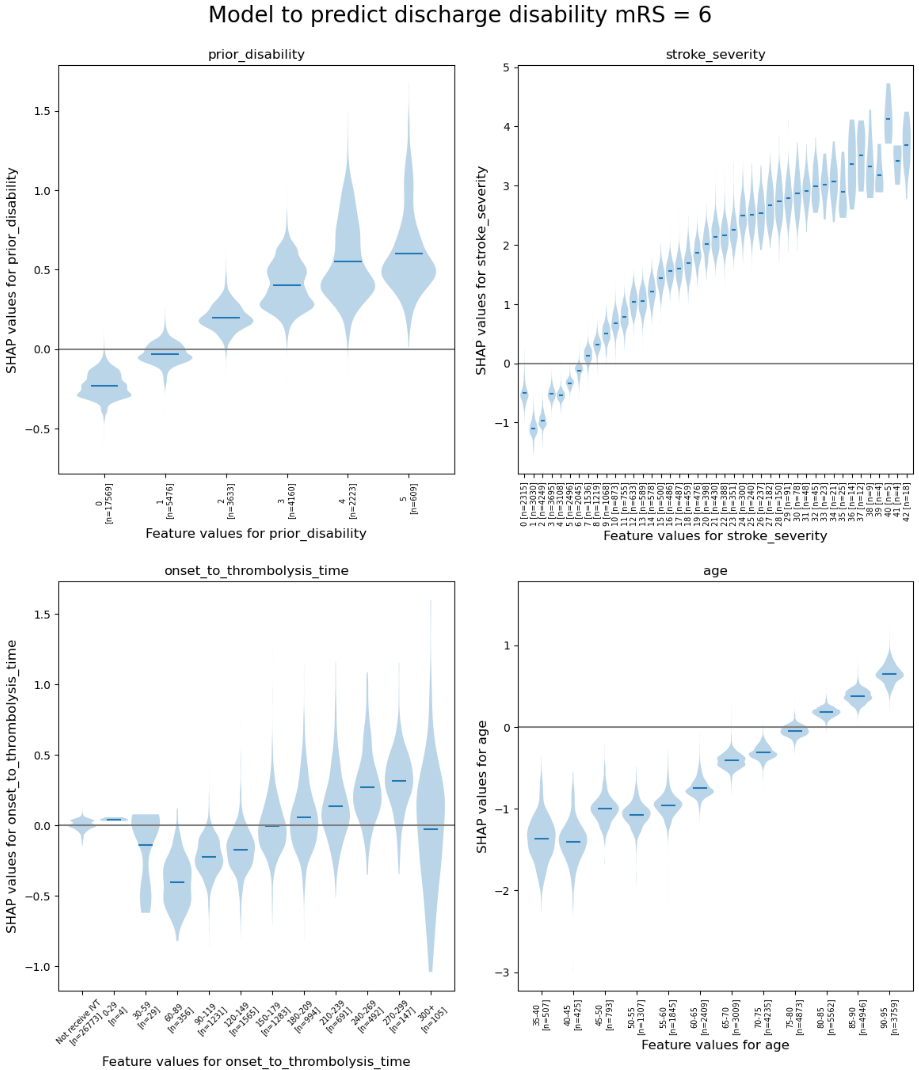
\includegraphics[width=0.75\textwidth]
    {./images/043_outcome_mrs6_violin_plots.png}\\
    \caption{}
    \label{fig:mrs6_violin}
\end{figure}

\begin{figure}[!h]
    \centering    
    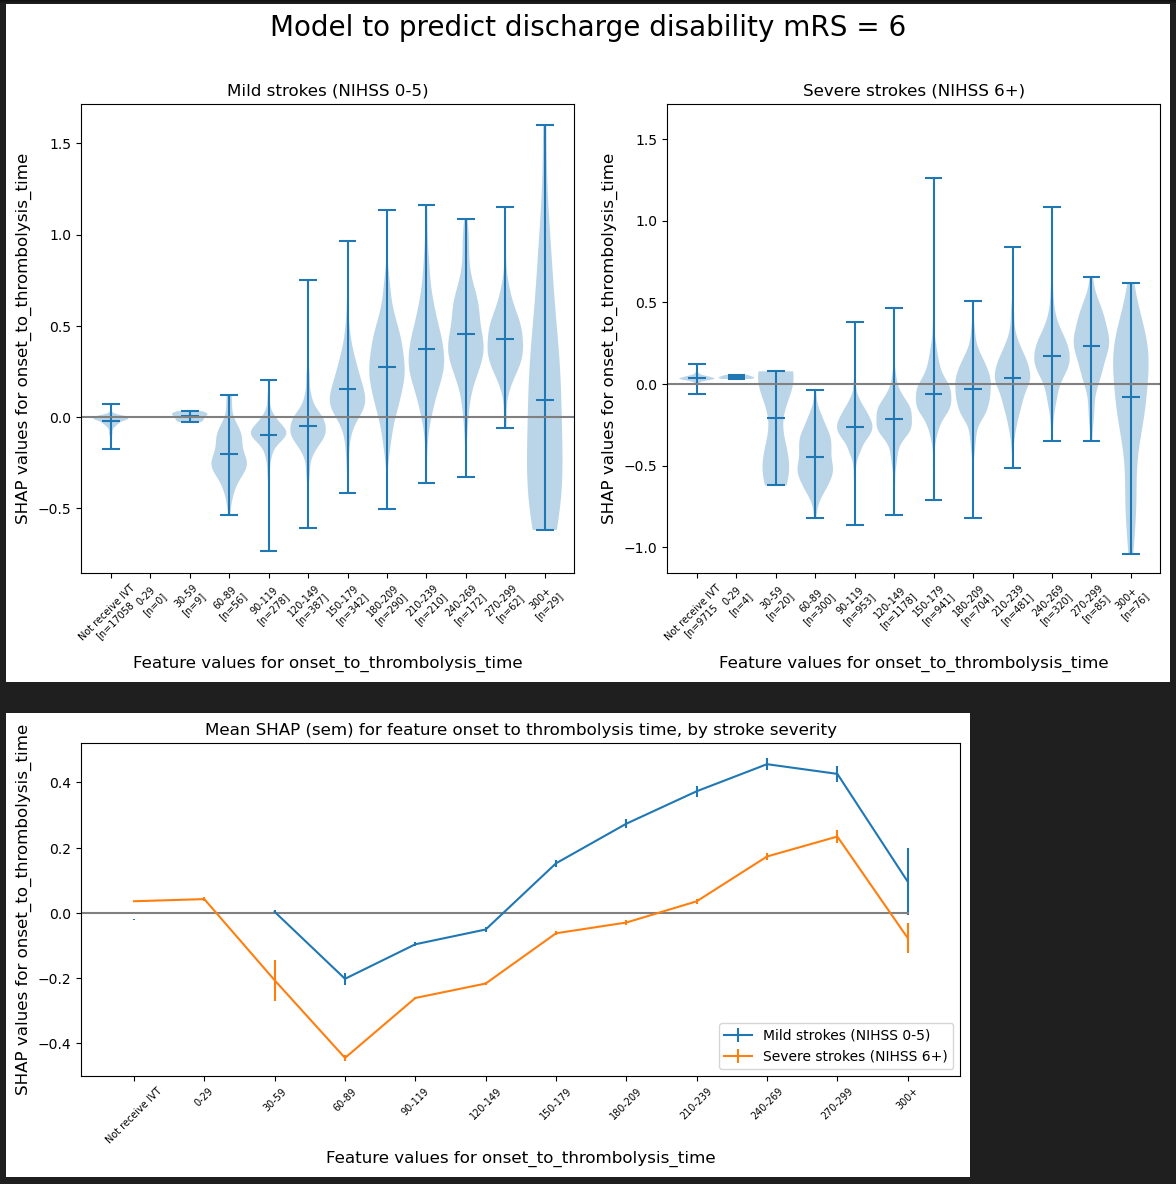
\includegraphics[width=0.75\textwidth]
{./images/053_predict_mrs6_split_by_ss.png}\\
    \caption{The impact of a feature value on the likelihood of death can be divided into subgroups. Here we see the effect of time to thrombolysis on likelihood of death for mild strokes (NIHSS0-5) and moderate and severe strokes (NIHSS 6+).}
    \label{fig:mrs6_violin_split}
\end{figure}




fig 2 caption: The impact of a feature value on the likelihood of death can be divided into subgroups. Here we see the effect of time to thrombolysis on likelihood of death for mild strokes (NIHSS0-5) and moderate and severe strokes (NIHSS 6+).


\begin{figure}[!h]
    \centering    
    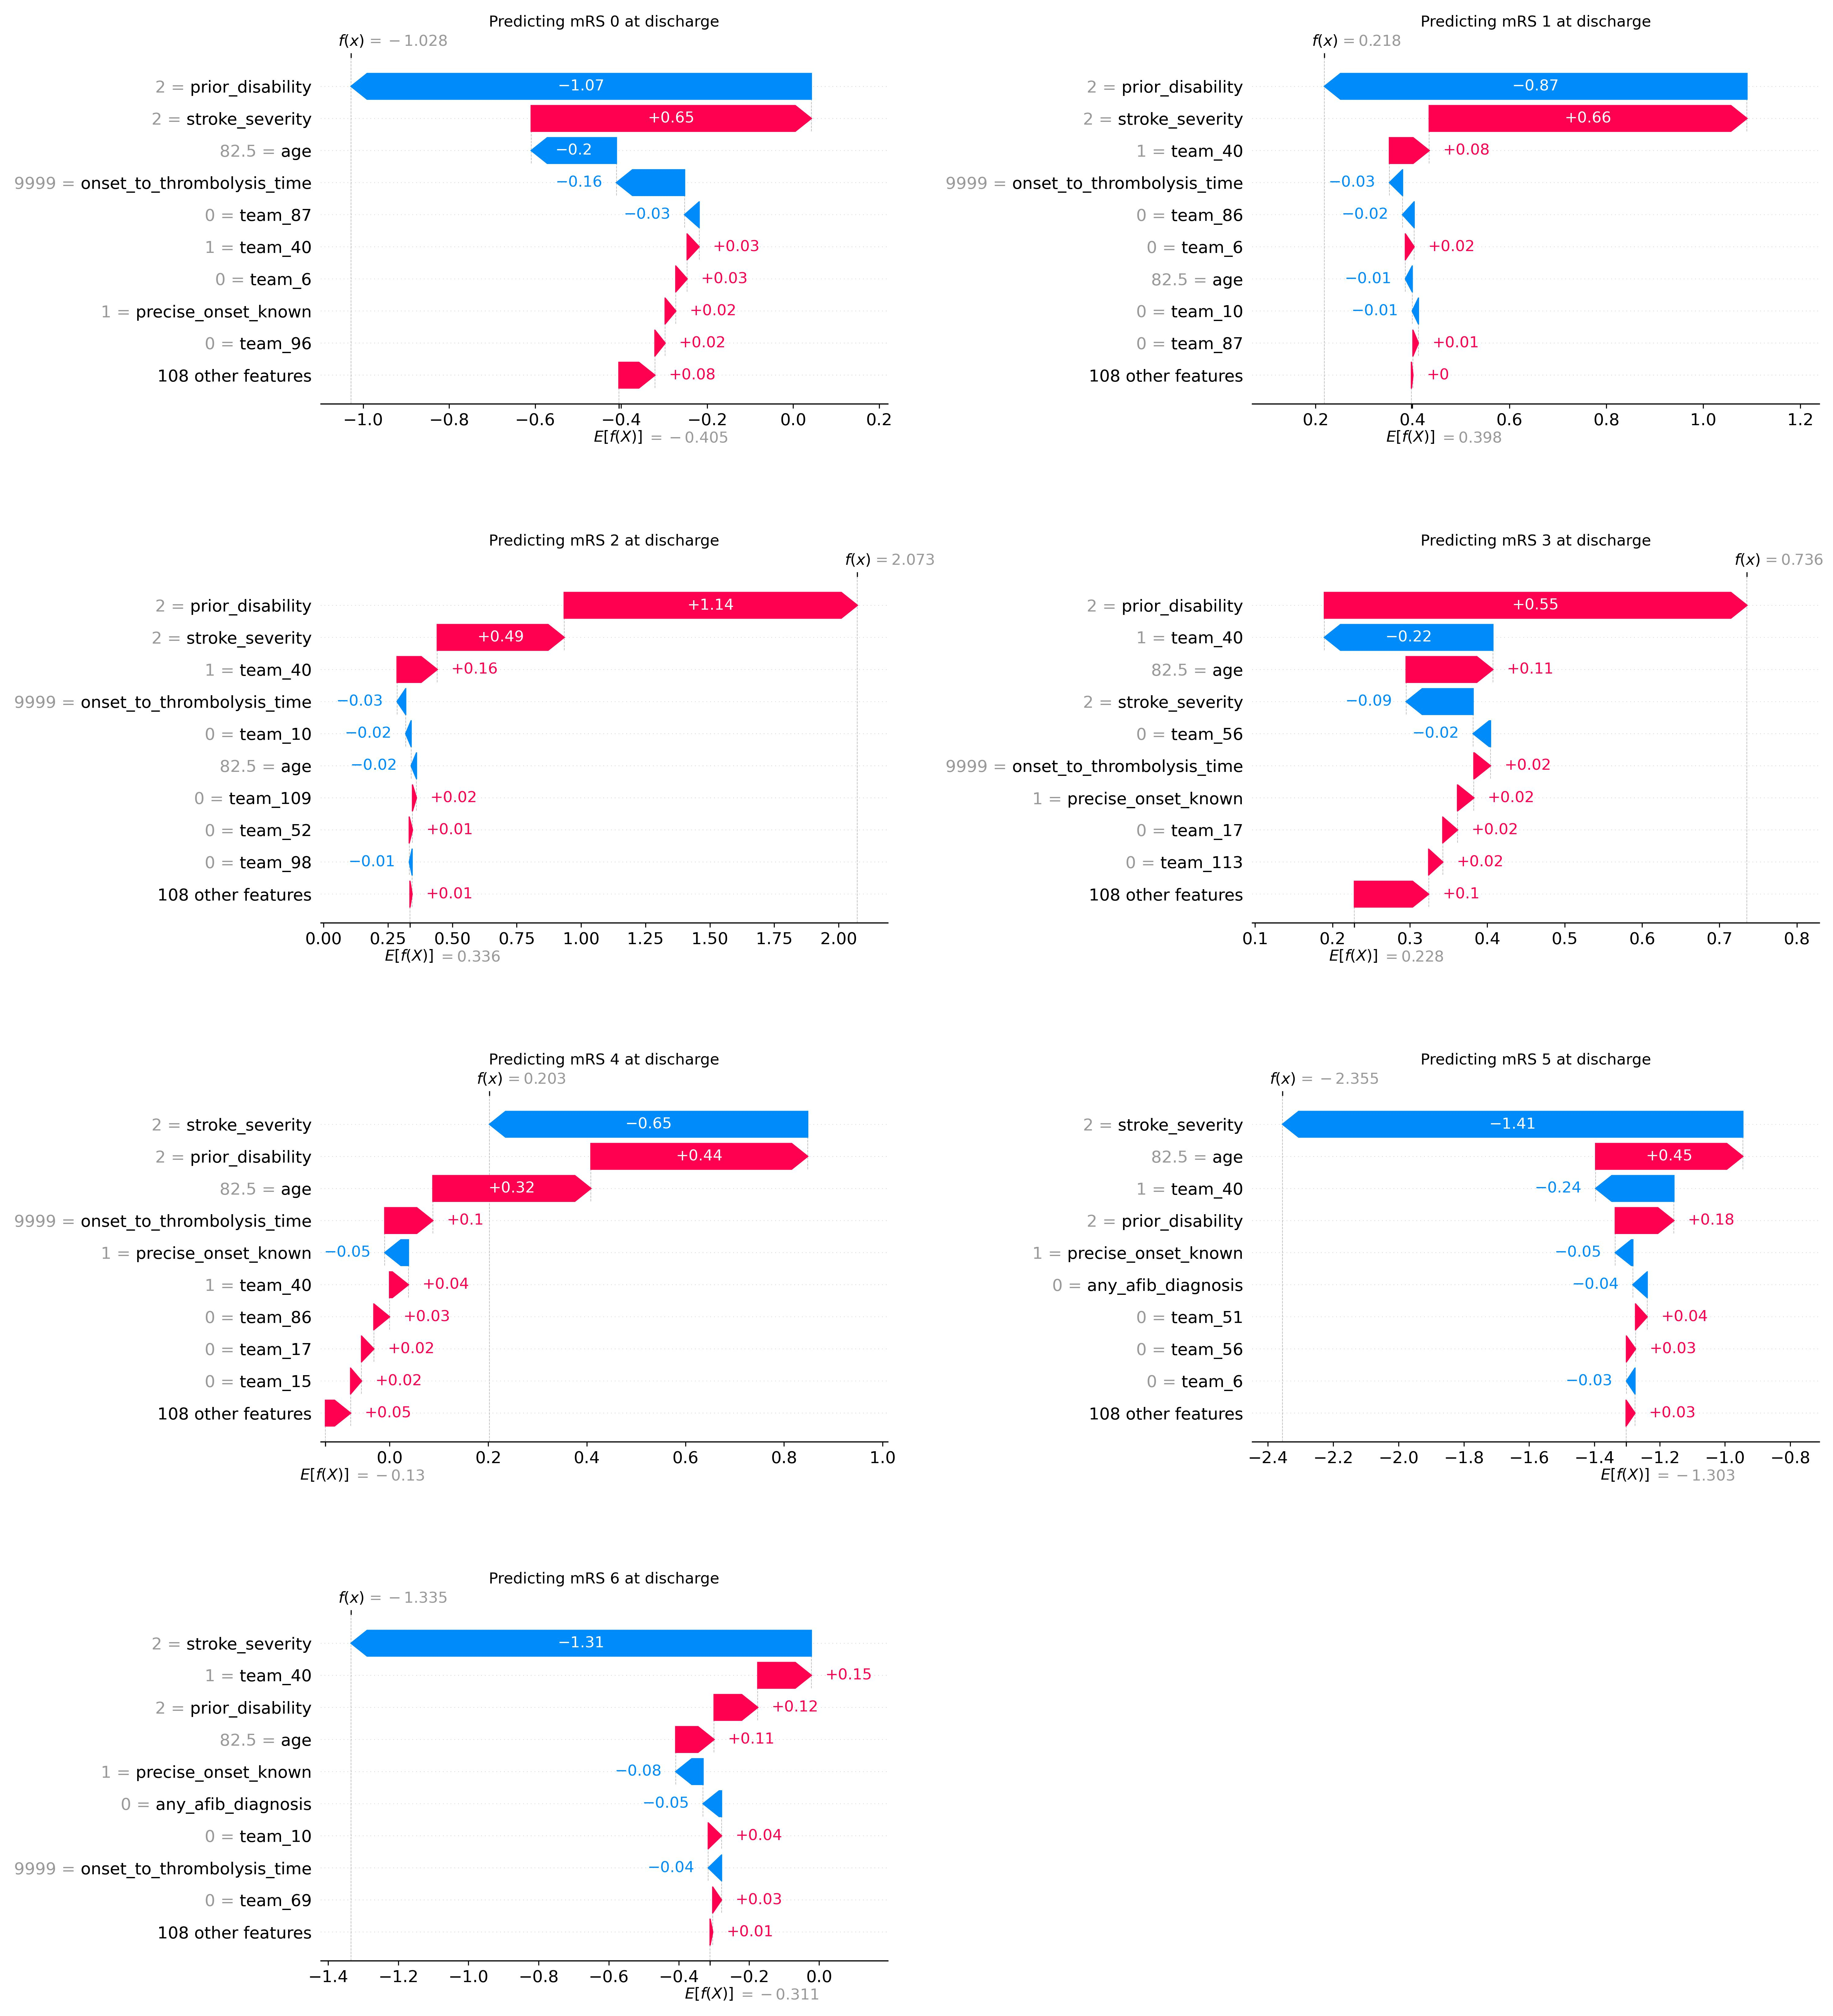
\includegraphics[width=0.75\textwidth]{./images/042_xgb_7_features_5fold_waterfall_for_each_class.jpg}\\
    \caption{Waterfall plots showing the influence of each feature on the predicted likelihood of a single patient having each level of mRS at discharge (top left displays mRS 0, through to bottom left displaying mRS 6). Each waterfall plot shows the SHAP base value (E|f(x)|) and the SHAP values for each of the input feature values, the sum of which equates to the overall likelihood for the patient being that mRS score at discharge (f(x)). The individual seven mRS predictions combine to create the mRS probability distribution at discharge for the patient (bottom right).
}
    \label{fig:results_waterfall_extra_words}
\end{figure}



FIGURE LAYOUT ABOVE AND BELOW RATHER THAN SIDE TO SIDE
\begin{figure}
    \centering
    \begin{subfigure}{1\textwidth}
      \centering
      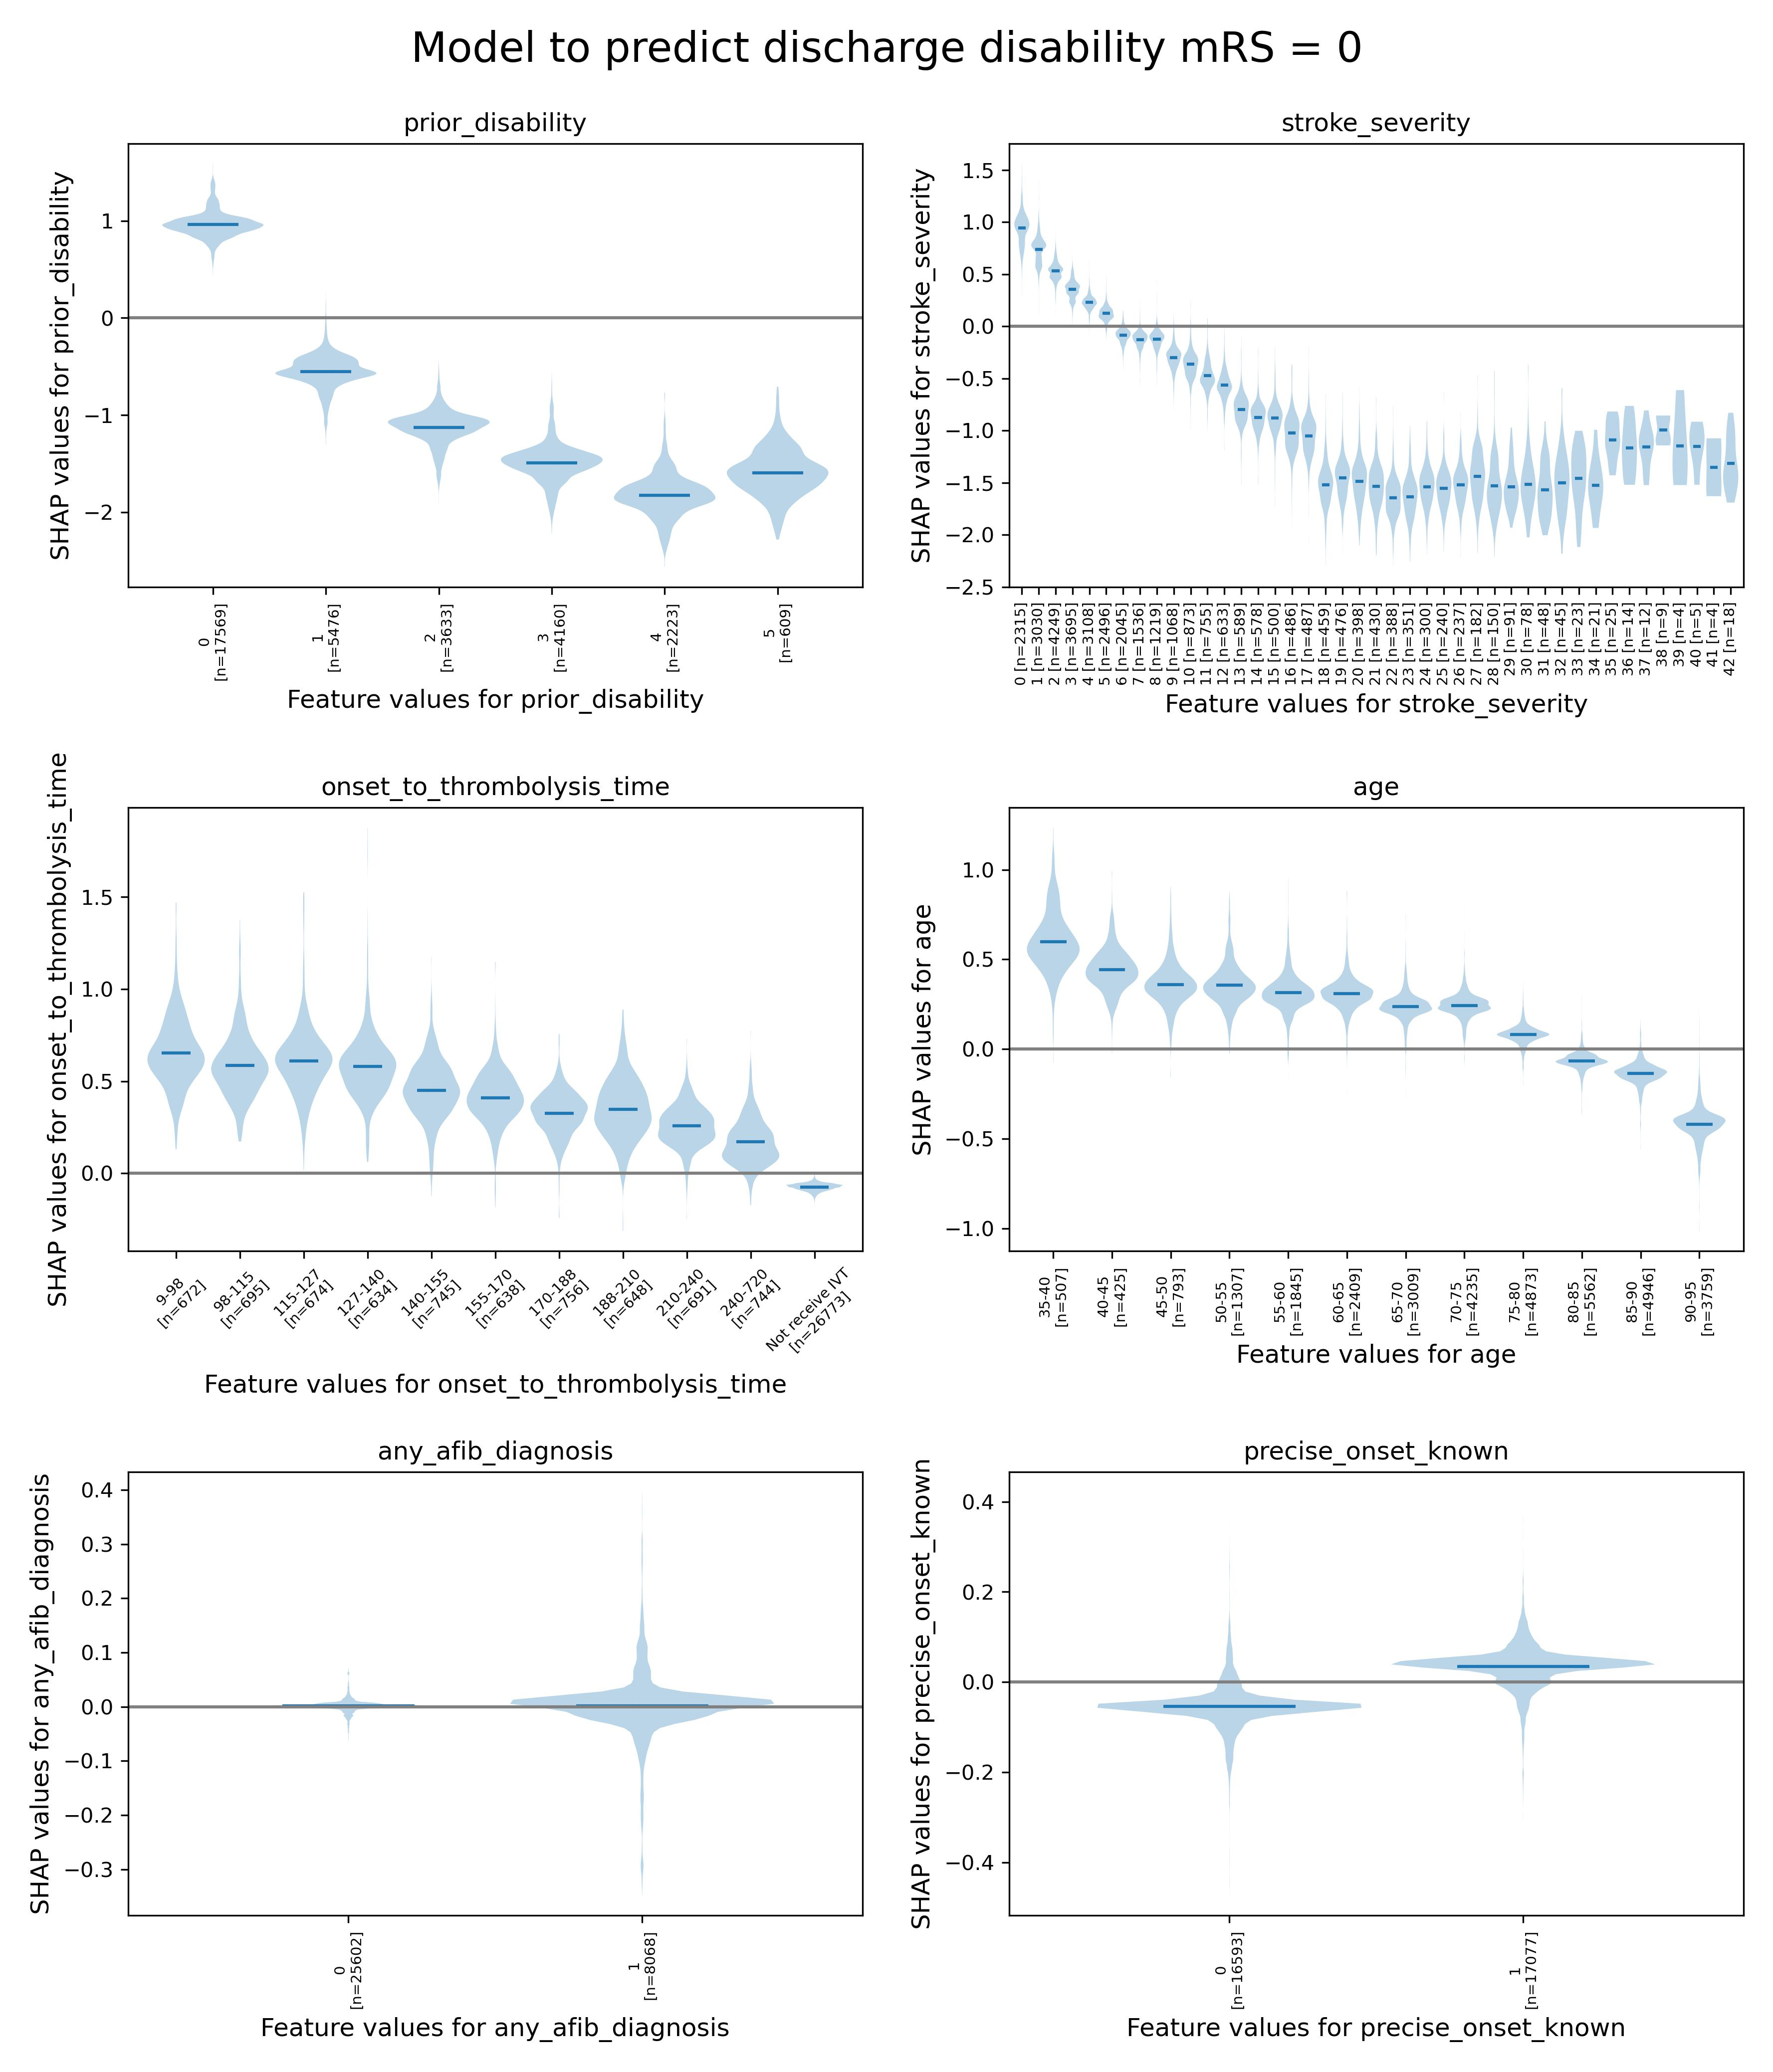
\includegraphics[trim={0 0 0 1.2cm}, clip, width=1\linewidth]    {./images/053_xgb_7_features_1fold_999999_thrombolysis_shap_violin_all_features_for_mRS0}\\
      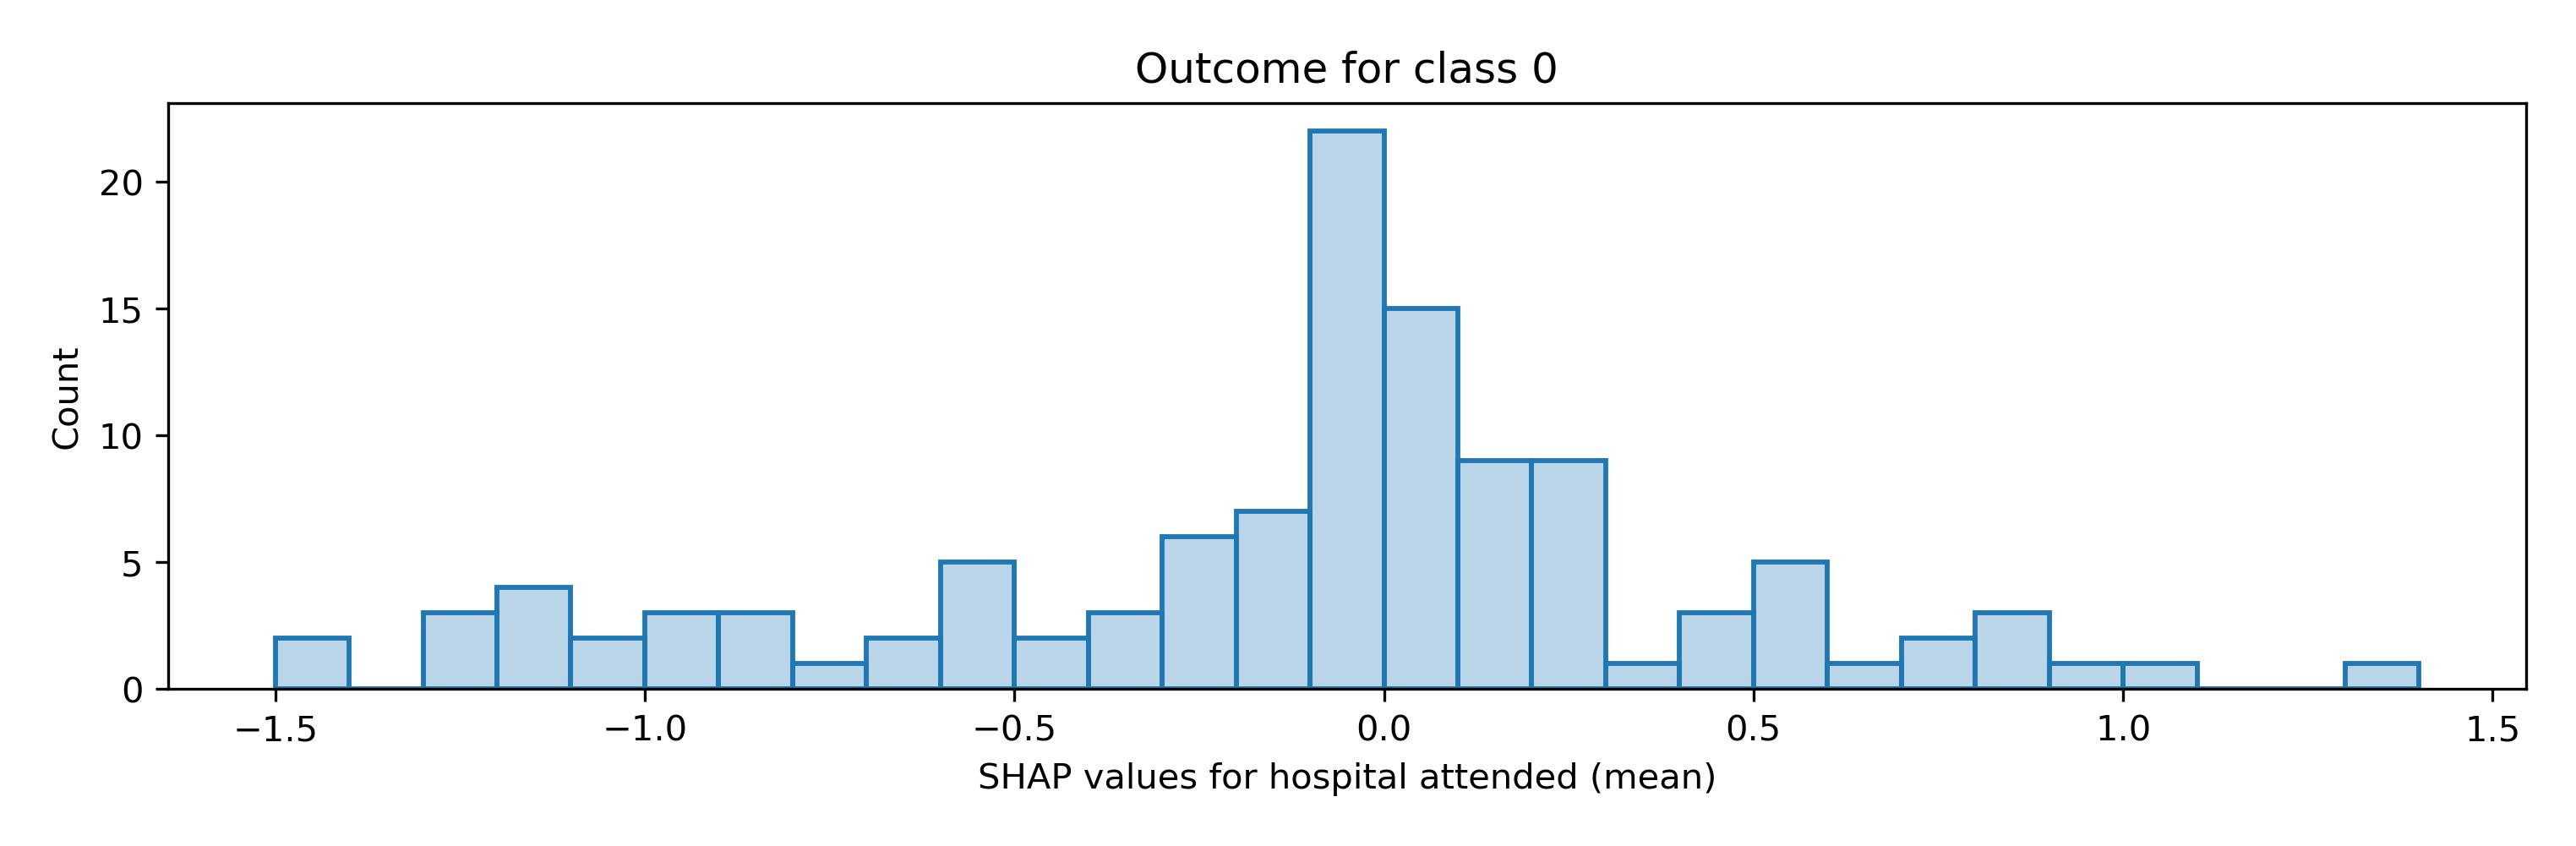
\includegraphics[trim={0 0 0 1cm}, clip, width=1\linewidth]    {./images/053_xgb_7_features_1fold_999999_hosp_shap_hist_mrs0}\\
      \caption{Predict the likelihood of no disability on discharge (mRS 6)}
      \label{fig:mrs_violin}
    \end{subfigure}%ults
\end{figure}
\begin{figure}\ContinuedFloat
    \centering
    \begin{subfigure}{1\textwidth}
      \centering
      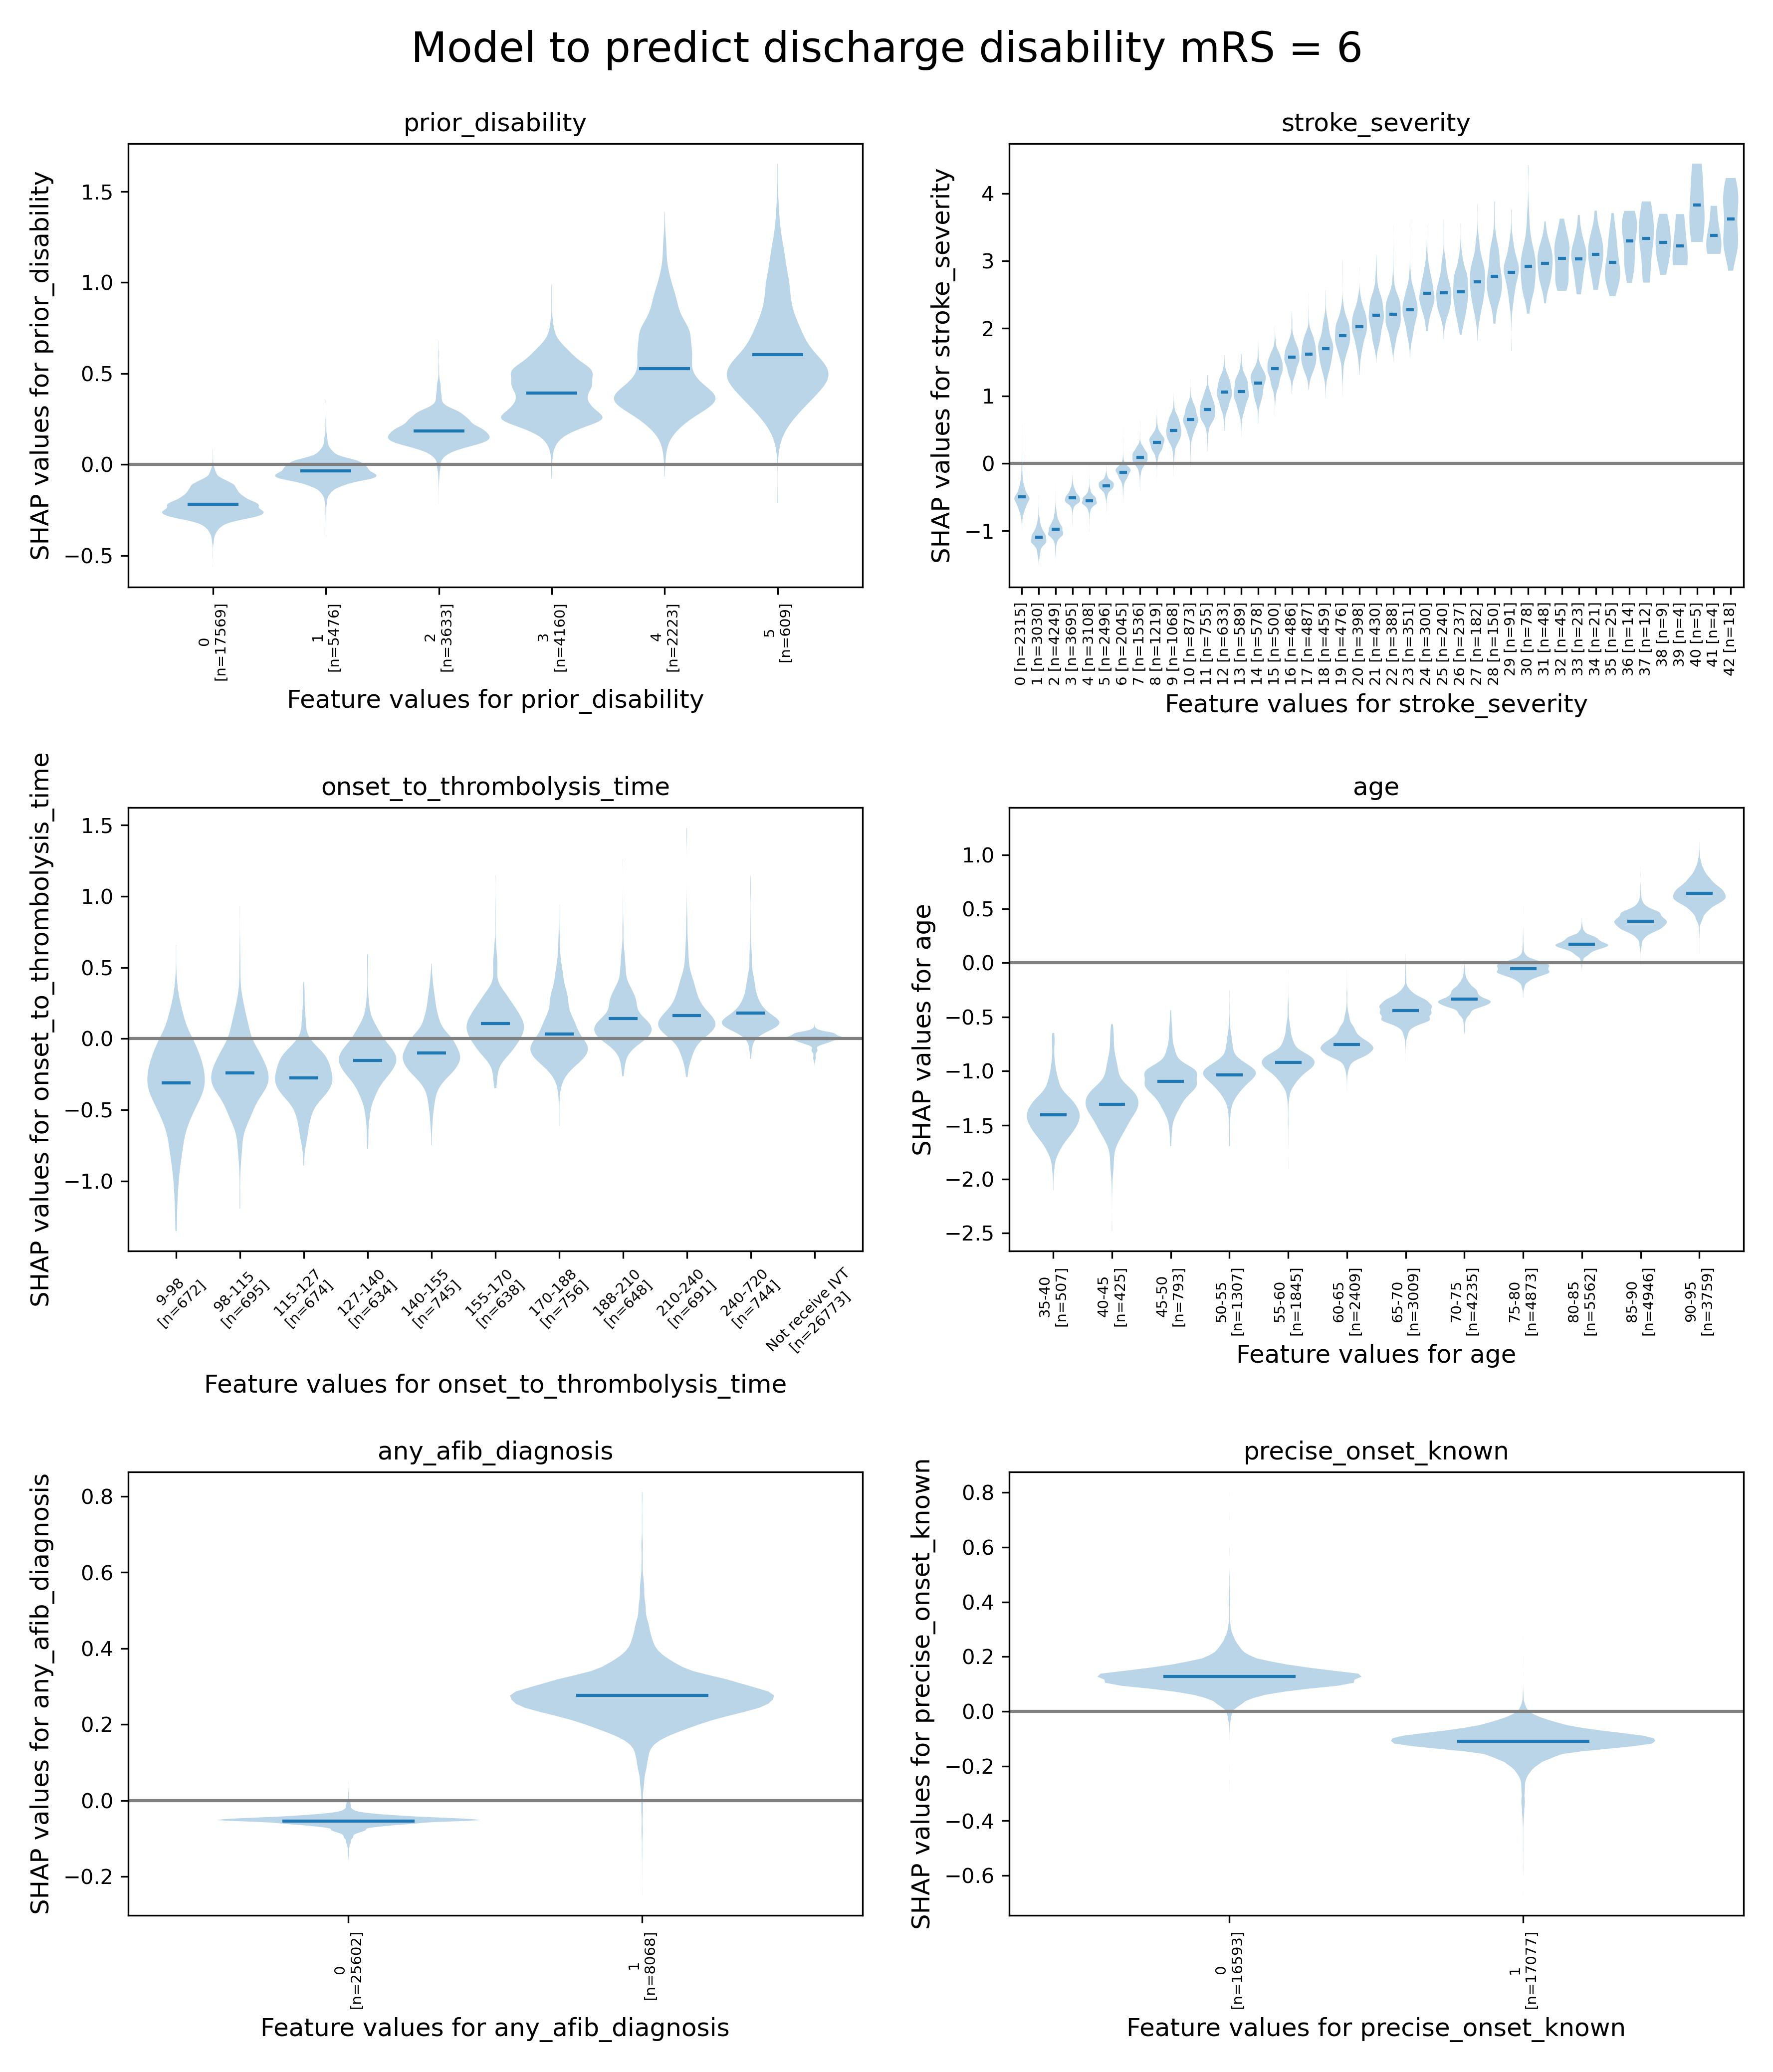
\includegraphics[trim={0 0 0 1.2cm}, clip, width=1\linewidth]{./images/053_xgb_7_features_1fold_999999_thrombolysis_shap_violin_all_features_for_mRS6}\\
      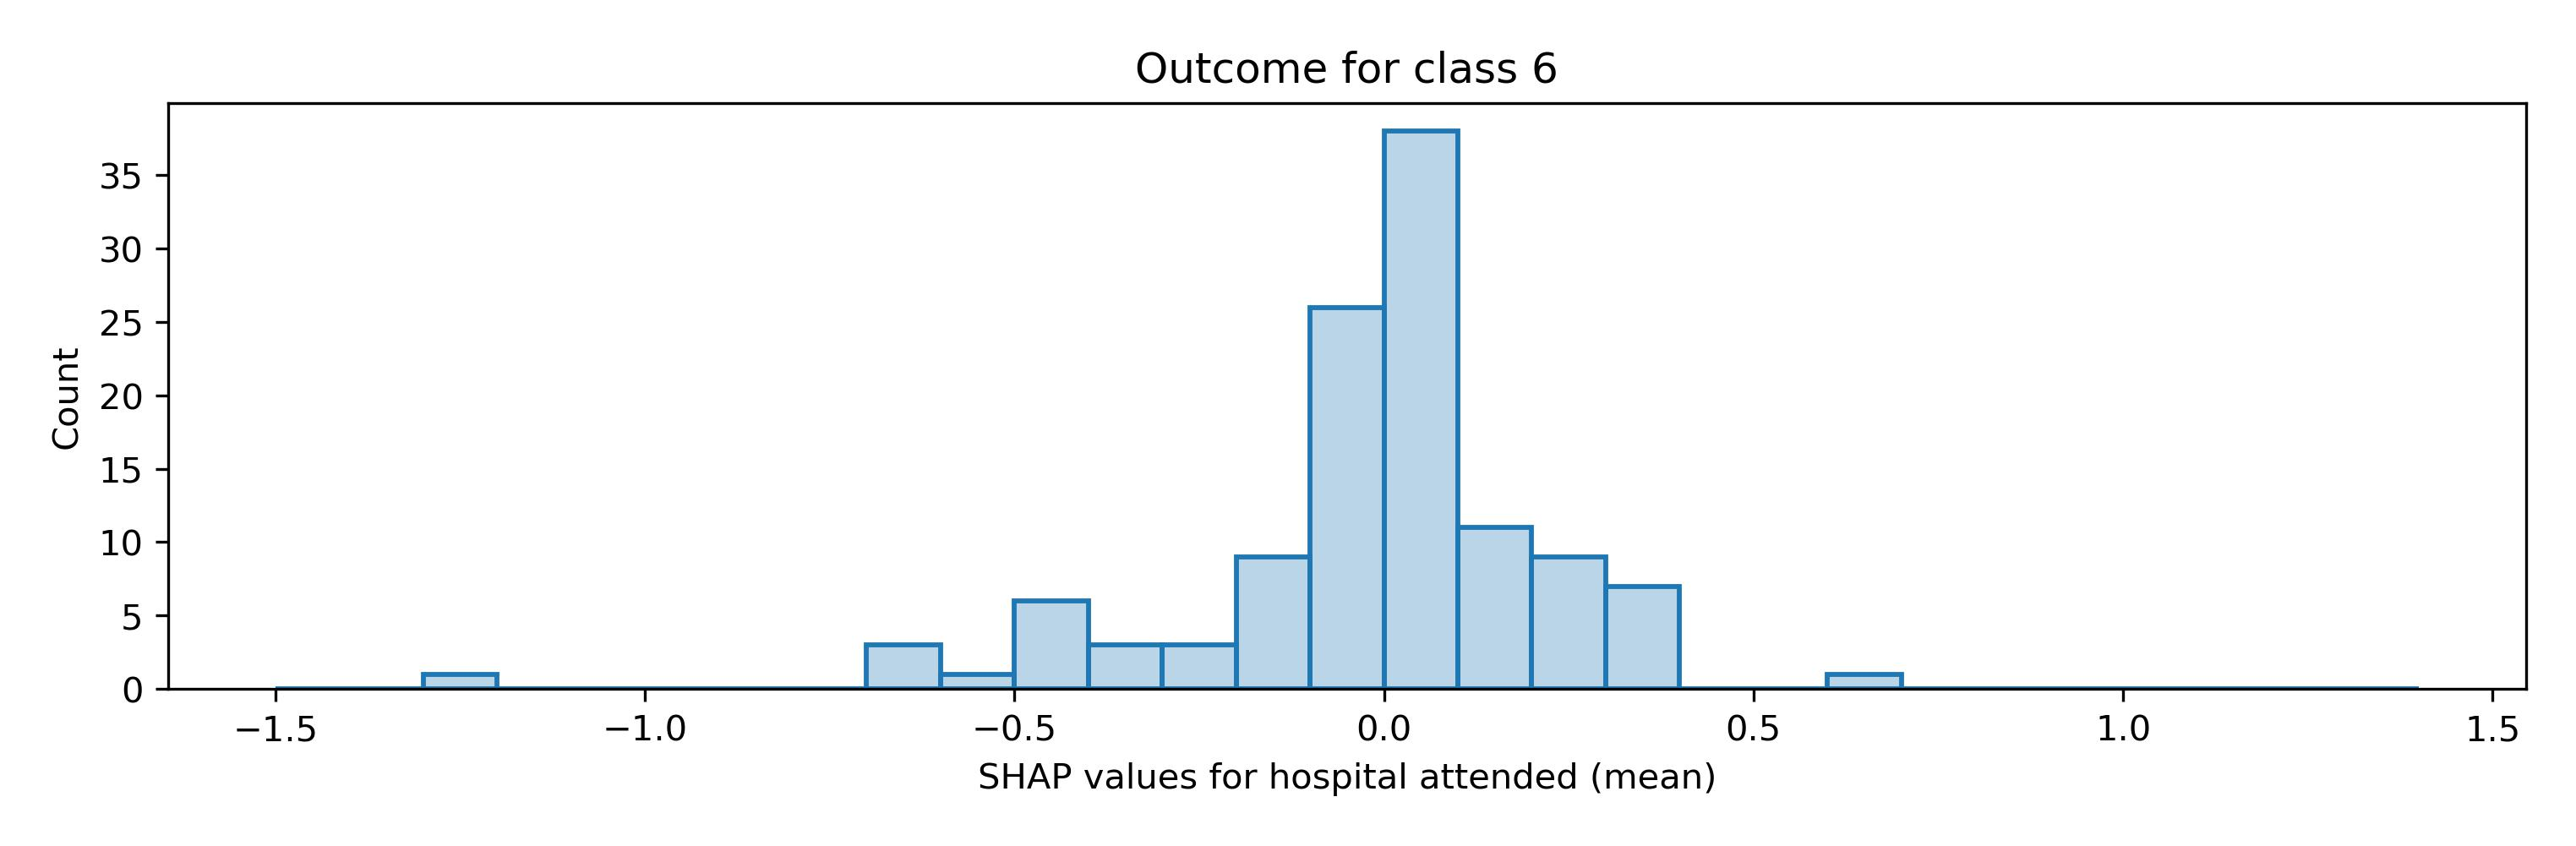
\includegraphics[trim={0 0 0 1cm}, clip, width=1\linewidth]    {./images/053_xgb_7_features_1fold_999999_hosp_shap_hist_mrs6}\\
      \caption{Predict the likelihood of death on discharge (mRS 6)}
      \label{fig:mrs_violin}
    \end{subfigure}%ults    
  \caption{Plots showing the relationship between SHAP values and feature values. Left: Predicting the likelihood of having no disability at discharge (mRS 0). Right: Predicting the likelihood of being dead at discharge (mRS 6). Top: Violin plots showing the relationship between SHAP values and feature values. The horizontal line shows the median SHAP value. The plots are ordered in ranked feature importance (using the mean absolute SHAP value across all instances). Bottom: Histogram showing the frequency of SHAP values for the hospital attended.}
    \label{fig:scatter}
\end{figure}


\section{Don't think including this as excluding high and low benchmark models}


WAS IN AS SECTION 4.5 (AFTER FIG 3 BAR CHARTS OF PROBABILITY DISTRIBUTIONS. THIS IS DISCUSSING CONNECT 4 FIGURE. CAN ALSO BE DISPLAYED AS A DONUT CHART)
\subsection{Comparing treatment decisions of the best outcome vs i) high and ii) low benchmark decisions}
(Including this section will need to include another model for treatment decisions, and take majority vote for the top and bottom 25 hospitals).

High benchmark hospitals are those 25 units with the highest IVT rate. Take majority vote and use that as the clinical decision in the model for all hospitals. This will result in giving thrombolysis to more people who we predict will get the better outcome from thrombolysis, but at the cost of more patients who we predict will not get the best outcome from thrombolysis. There's a trade-off of benefiting more people at a smaller increase in causing potential harm from IVT. 

The orange dots are those patients who could benefit but not receive thrombolysis, so the high benchmark hospital majority vote is still missing some patients that we predict could have a better outcome with thrombolysis.

We can also do the opposite, taking the 25 least IVT units and use their majority vote. We see there are more orange dots (not given IVT but expected to have a good outcome), and more white dots (not given and no benefit), showing that the low benchmark vote misses more people who could get benefit yet does not give treatment to those who would not benefit. Green dots are reduced (receives IVT and good outcome), and purple dots are reduced (receives IVT and bad outcome), showing that they are not giving IVT as much patients, and so miss benefit as well as missing harm.

To get the most benefit you can increase risk of harm. There appears to be a trade-off.


\section{SHAP for matchign treatment when using full dattaset, and not just the test set for first kfold + MT patients}


\textbf{Violin plots}
Illustrate this with a violin plot. Figure \ref{fig:shap_violin_all_benefit_ivt} shows patients who should benefit from treatment. What is it about the patients that means they didn't receive it, but would have benefited from treatment?

\begin{figure}
\subfloat[]{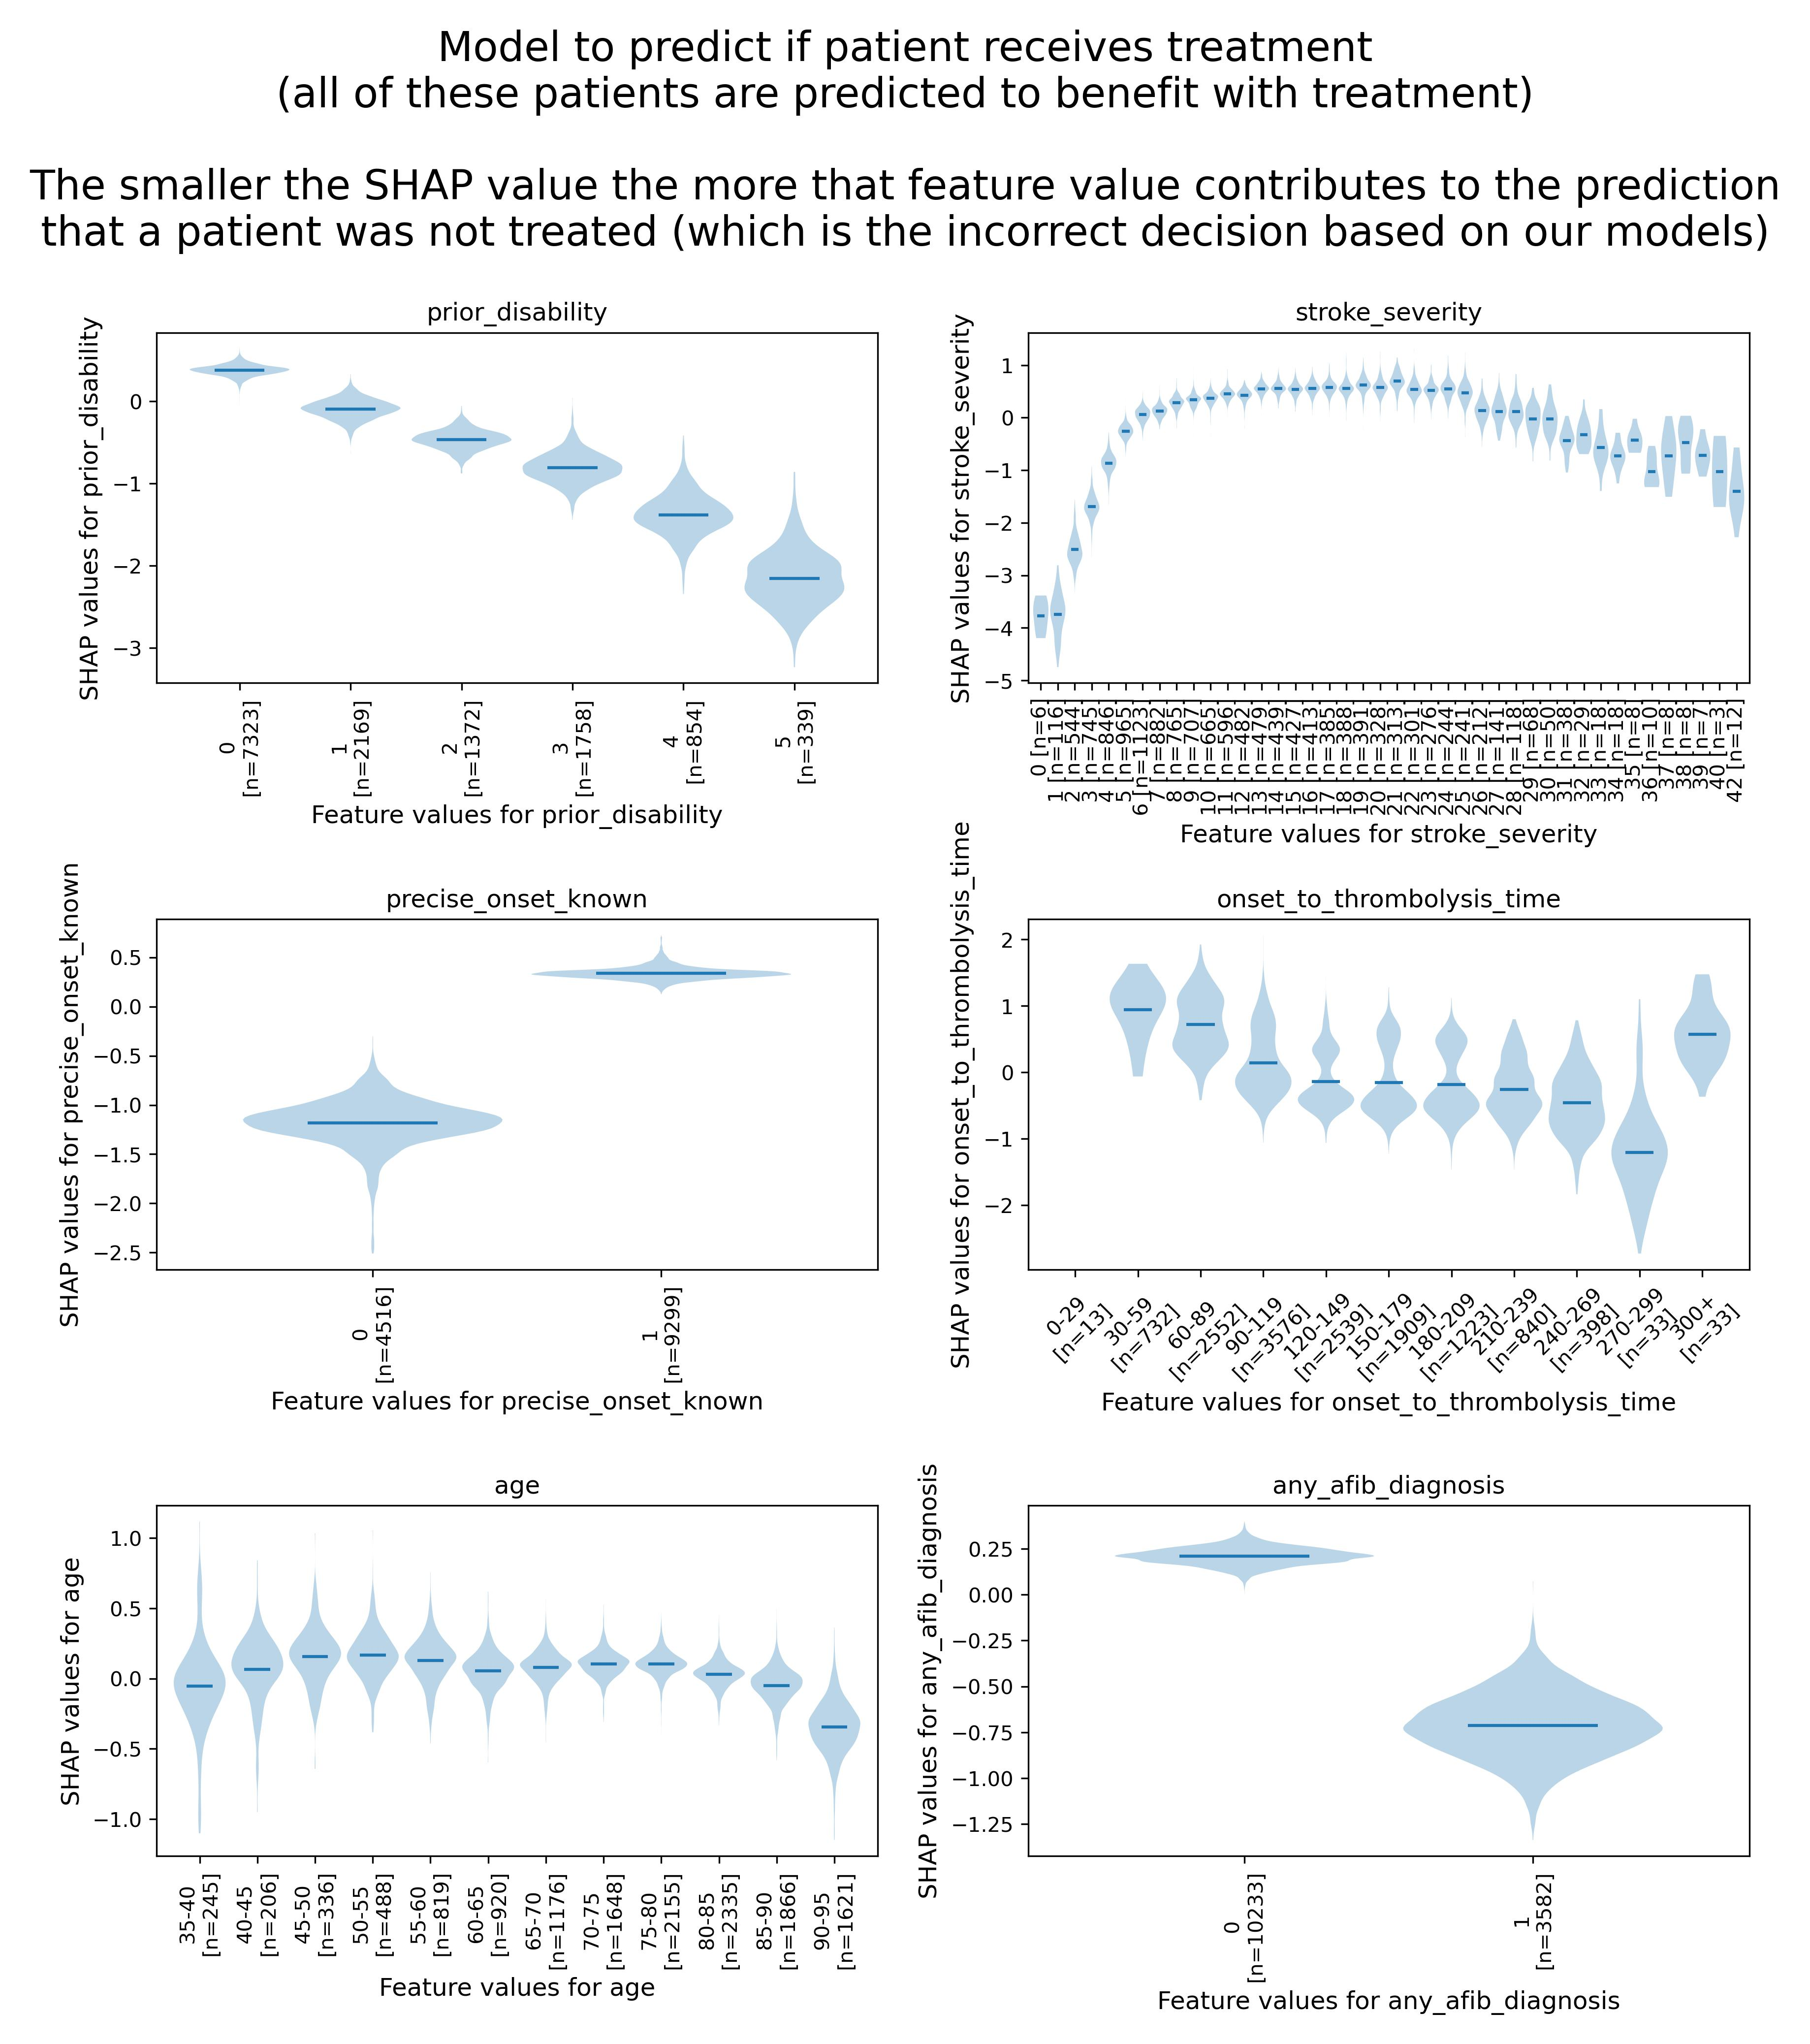
\includegraphics[width = 5in]{./images/218_shap_violin_all_benefit_with_ivt_Lowest_weighted_mrs_and_least_mrs5_6_Actual_treatment.jpg}}\\
\caption{}
\label{fig:shap_violin_all_benefit_ivt}
\end{figure}

\ref{fig:shap_violin_none_benefit_ivt} shows patients who should not benefit from treatment. What is it about the patients that means they received it, but would have benefited from not receiving treatment?

\begin{figure}
\subfloat[]{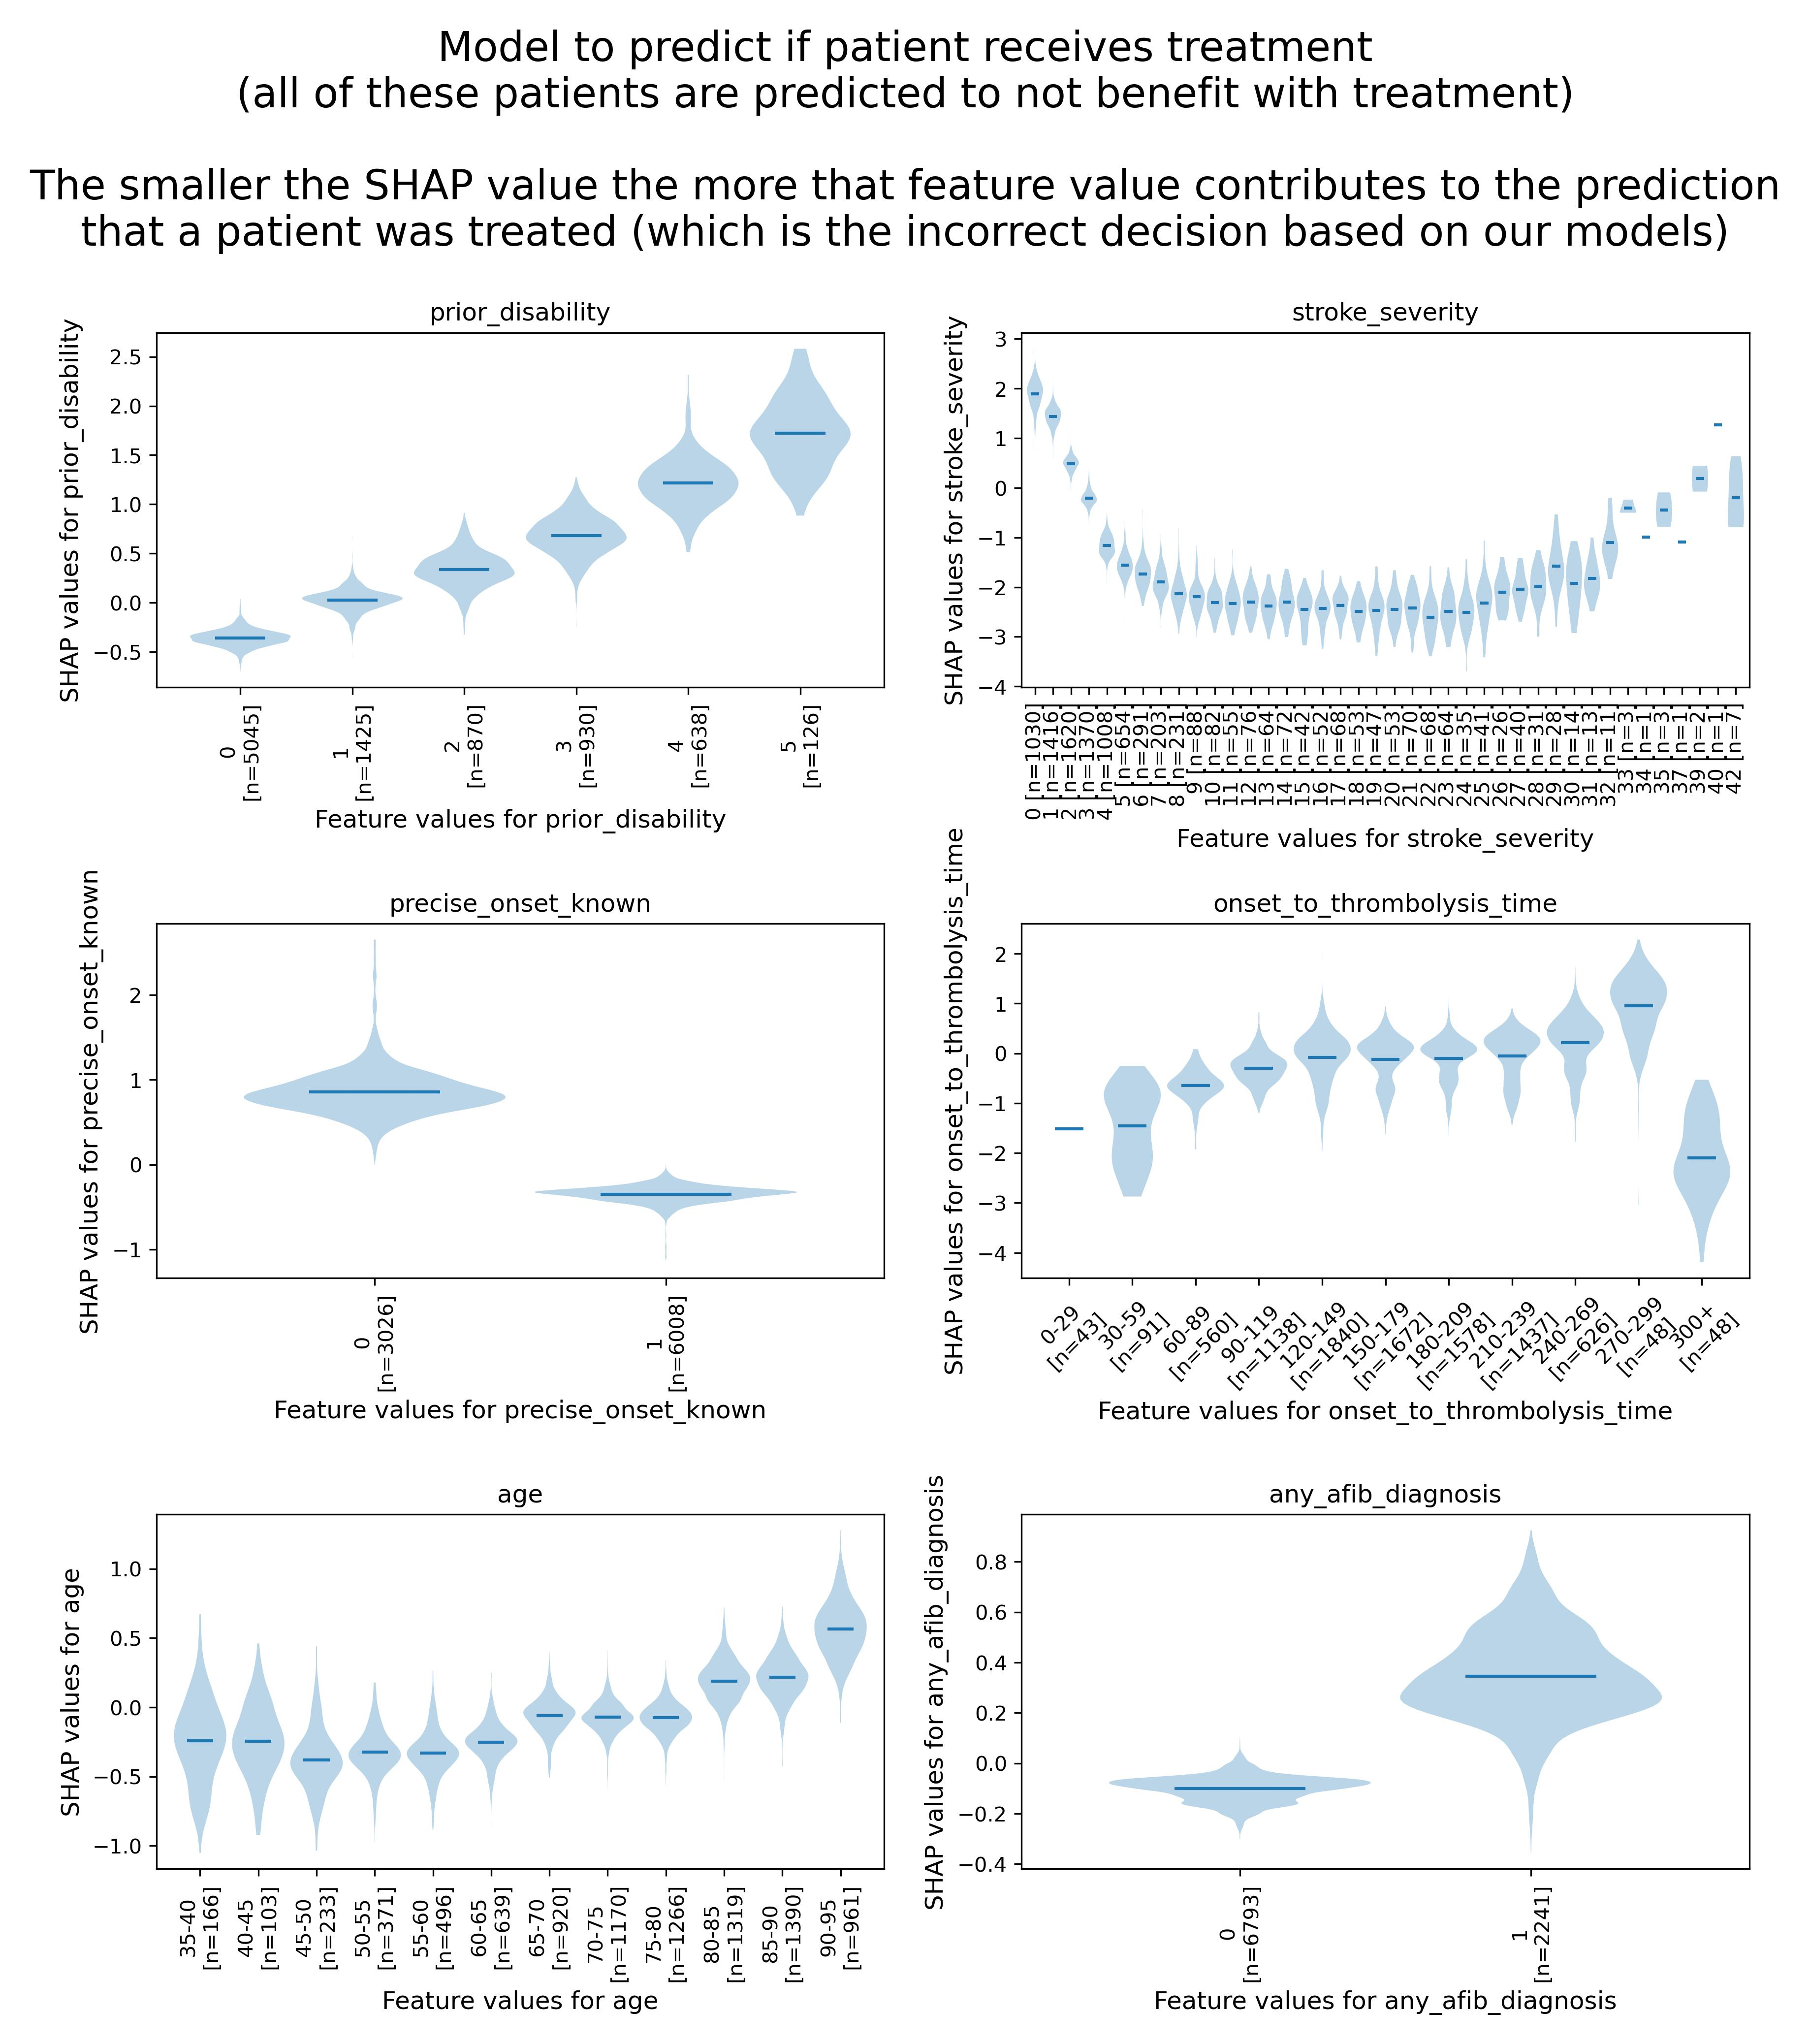
\includegraphics[width = 5in]{./images/218_shap_violin_none_benefit_with_ivt_Lowest_weighted_mrs_and_least_mrs5_6_Actual_treatment.jpg}}\\
\caption{}
\label{fig:shap_violin_none_benefit_ivt}
\end{figure}

See the points as relative, as zero means it is not shifting model from base SHAP.

Safest bet of the best outcome with treatment, choose a patient with ideal characteristics (these are younger, no AF, early IVT, SS 10-25).

These ideal characteristic values also identify patients that have been given thrombolysis but are predicted to not have the best outcome with treatment. So we can't say always give it to a single certain characteristic value, as need to take into account all characteristics.

So a drug label contains a list of ideal characteristics - if you follow this then you miss benefit. 

In order to recognise those patients who would, and would not, you need a model to combine all the characteristics. It's combination of characteristics, not a single value. No simple rules to recognise patients who should be treated but aren't currently receiving treatment (and vice versa).

On the flip side, non-ideal characteristic values (such as older, AF, later IVT, SS mild or severe) help to identify patients that have not been given thrombolysis but are predicted to have the best outcome with treatment.

All of this points back to needing a model.

The model takes into account prior disability 


VALUES BEFORE ADJUST FOR ATRIAL FIBRILLATION ANTICOAGULANTS.
Of the 36,605 patients that received thrombolysis, 28,243 patients were predicted to have a better outcome with thromboylsis, 8,362 patients were not predicted to have a better outcome with thromboylsis.
Of the 354,789 patients that did not receive thrombolysis, 27,017 patients were predicted to have a better outcome with thromboylsis, 27,772 patients were not predicted to have a better outcome with thromboylsis.




Patients on atrial fibrilation anticoagulants presents an additional risk of a bleed, and so any patient given thrombolysis and on anticoagulants may have had some additional tests. The dataset does not capture this information, therefore, for patients on anticoagulants that did not receive thrombolysis, We take the cautious approach and remove patients on atrial fibrilation anticoagulants that are not given thrombolysis from this analysis, otherwise we could overestimate the benefit of thrombolysis. This effects ??1165 patients (of the ??20,825 patients) that are on anticoagulants.





\iffalse
The venn diagram (figure \ref{fig:venn_actual_best}) shows the overlap of patients that were actually treated and those that were only treated if it was predicted to give them the best outcome.
Venn diagram showing what happens to 100 average patients, each arrive within 4 hours known onset. Did they receive IVT, and compare this with whether it was the best decision for each of them - do this by using the counterfactual model and calculating what would your outcome be with/without IVT). Comforting there's an overlap of who should and who are treated. But those Yellow and blue patients are hard to identify using some binary labels. Decision is shall I risk being in the yellow or blue circle.


\begin{figure}
{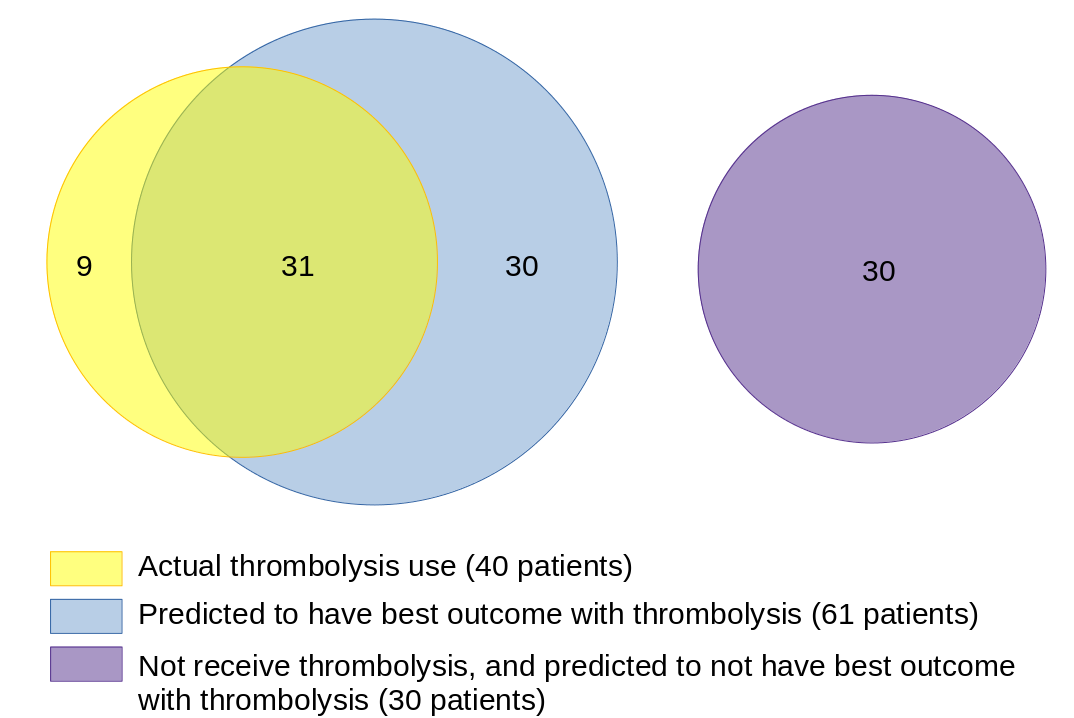
\includegraphics[width = 5in]{./images/impress_venn_diagram_for_paper.png}}\\ %218_venn_diagram_slide.png}}\\
\caption{Venn diagram comparing two options for making the decision to give thrombolysis to 100 average patients (each arrive within 4 hours of known onset): 1) the actual thrombolysis decision 2) the models prediction that the best outcome is with thrombolysis.}
\label{fig:venn_actual_best}
\end{figure}

\fi



%{./images/210_xgb_all_data_multiclass_outcome_999999_scatter_criteria_not_treated}%210_better_outcome_criteria_scatter_not_treated.png}

%{./images/210_xgb_all_data_multiclass_outcome_999999_scatter_criteria_treated}%210_better_outcome_criteria_scatter_treated.png}

\iffalse

\subsection{\textit{Matching treatment} models: Accuracy}

The treatment decision matches the predicted best treatment decision. Accuracy for predicting treatment for patients that "should be treated" was 74.3\%, and 83.1\% for predicting treatment for patients that "should not be treated". ROCAUC was 0.788 and 0.814 respectively.

The Appendix contains further model accuracy analysis.

\fi





\section{Method}

\subsection{Data}

Data were retrieved for 168,347 emergency stroke admissions to acute stroke teams in England for six years, 2016–2021 (inclusive), obtained from the Sentinel Stroke National Audit Programme (SSNAP). Data fields were provided for the hyper-acute phase of the stroke pathway, up to and including our target feature: disability on inpatient discharge. Disability is recorded in the SSNAP dataset using the modified Rankin Scale (mRS), where mRS 0 represents perfect health and mRS 6 represents death. The data includes 118 acute stroke hospitals (each has at least 250 stroke admissions and delivers thrombolysis to at least 10 patients in the six years).

\subsection{Machine learning models}
For the different patient outcome analysis included in this paper, we trained two XGBoost models to predict various target features from the other feature values that describe the patients pathway, the patients characteristics and the attended hospital. For a new instance (in our case, a new patient) the model predicts based on what it has seen before. Each analysis in the paper will refer to the model used:
\begin{enumerate}
    \item \textit{Multiclass outcome} model [target feature: mRS score at discharge]: A multiclass classification model to predict the likelihood of each level of disability at discharge for each patient who had a stroke. Multiclass classification models can be thought of as a set of models (one for each target class) that gives the probability for that class (in our case, for each mRS score), such that the sum of the probabilities equals one (known as softmax). The model, therefore, reports a probability distribution across the seven mRS levels for each patient. Train using a 5-fold train-test cross validation used to test the accuracy of the model, for feature selection, and to test reproducibility of SHAP values. The model fitted on the first k-fold is used to investigate the relationship between feature values and predictions. If a prediction for a single mRS level is required, the model will predict that the patient has the mRS level with the highest probability.

    Using the \textit{multiclass outcome} model to predict the counterfactual outcomes for each patient (whether they did, and did not, receive thrombolysis) we can translate the two probability distributions obtained into a binary feature to represent whether the patient is predicted to have a better outcome receiving thrombolysis. For those patients that received thrombolysis, create the counterfactual case by setting the feature onset to treatment time to -100 (to predict what their disability at discharge probability is without treatment). For those patients that were not given thrombolysis create the counterfactual case by assuming their scan to thrombolysis time (which is not recorded) is the median of the attended hospital, and set the feature onset to treatment time as the sum of the recorded pathway durations (onset to arrival and arrival to scan) and the median scan to thrombolysis time of the attended hospital. We use a cautious definition (containing two criteria which both must be met) to determine whether a patient has a better outcome with treatment: 1) on average reduce disability, 2) without increasing the risk of death and the severest disability (mRS 5+).
    
    \begin{itemize}
        \item \textit{Calculate new target feature: Patient received treatment decision predicted to give better outcome}. We can define a binary target feature where 0 represents not matching (predicted vs actual), and 1 represents a match by comparing the prediction of whether a patient would have a better outcome with treatment, with their actual treatment received.
    \end{itemize}
    
    \item \textit{Matching treatment} model [target feature: patient received treatment decision predicted to give better outcome]: A model to predict the binary target of whether the patient received the treatment decision that was predicted to give them the better outcome (where the binary target feature value of 0 represents not matching, and 1 represents matching). We train two separate models using two different patient sub-populations: i. patients with a predicted better outcome with thrombolysis ii. patients not predicted to get a better outcome with thrombolysis. 
    
    Use this model (and their associated SHAP values) to explore what patient characteristics contribute to a wrong treatment decision (based on the predicted best outcome). This will inform which patients to change behaviour for: those to instead leave alone when otherwise, and those to instead give treatment. To aid interpretability, convert the SHAP values to sensitivity of treatment (proportion of patients who would benefit from treatment who are treated), and specificity of treatment (proportion of patients who would not benefit from treatment who are not treated):

        INCLUDE EQUATION HERE
    
\end{enumerate}



\iffalse

Figure \ref{fig:shap_matching_treatment} shows the SHAP values for the two \textit{matching treatment} models, that explain the contribution of the feature values to an incorrect treatment decision (based on the \textit{multiclass outcome} model prediction).

Figure \ref{fig:shap_matching_treatment_should} shows patients who should benefit from treatment. What is it about the patients that means they didn't receive it, but would have benefited from treatment?
Figure \ref{fig:shap_matching_treatment_should_not} shows patients who should not benefit from treatment. What is it about the patients that means they received it, but would have benefited from not receiving treatment?

Interpret the SHAP values as relative - where zero means that the feature value is not contributing to moving the prediction away from the default, base, SHAP value. We know that an ideal patient to get the best outcome with treatment has these ideal characteristics: younger, no atrial fibrilation diagnosis, early treatment,  a moderately mild stroke severity, precisely known onset time, and no prior disability. Figure \ref{fig:shap_matching_treatment_should_not} shows that these ideal characteristic values also identify the patients that have been given thrombolysis but are predicted to not have the best outcome with treatment. So treatment is not always beneficial for patients that satisfy a single characteristic value. We need to take the combination of characteristics into account. Conversely, \ref{fig:shap_matching_treatment_should} shows that the non-ideal characteristic values (such as older, later treatment, mild or severe stroke severity, prior disability, and non precise onset time, each help to identify patients that have not been given thrombolysis but are predicted to have the best outcome with treatment.

\begin{figure}
    \centering
    \begin{subfigure}{.5\textwidth}
      \centering
      \captionsetup{width=.9\linewidth}
      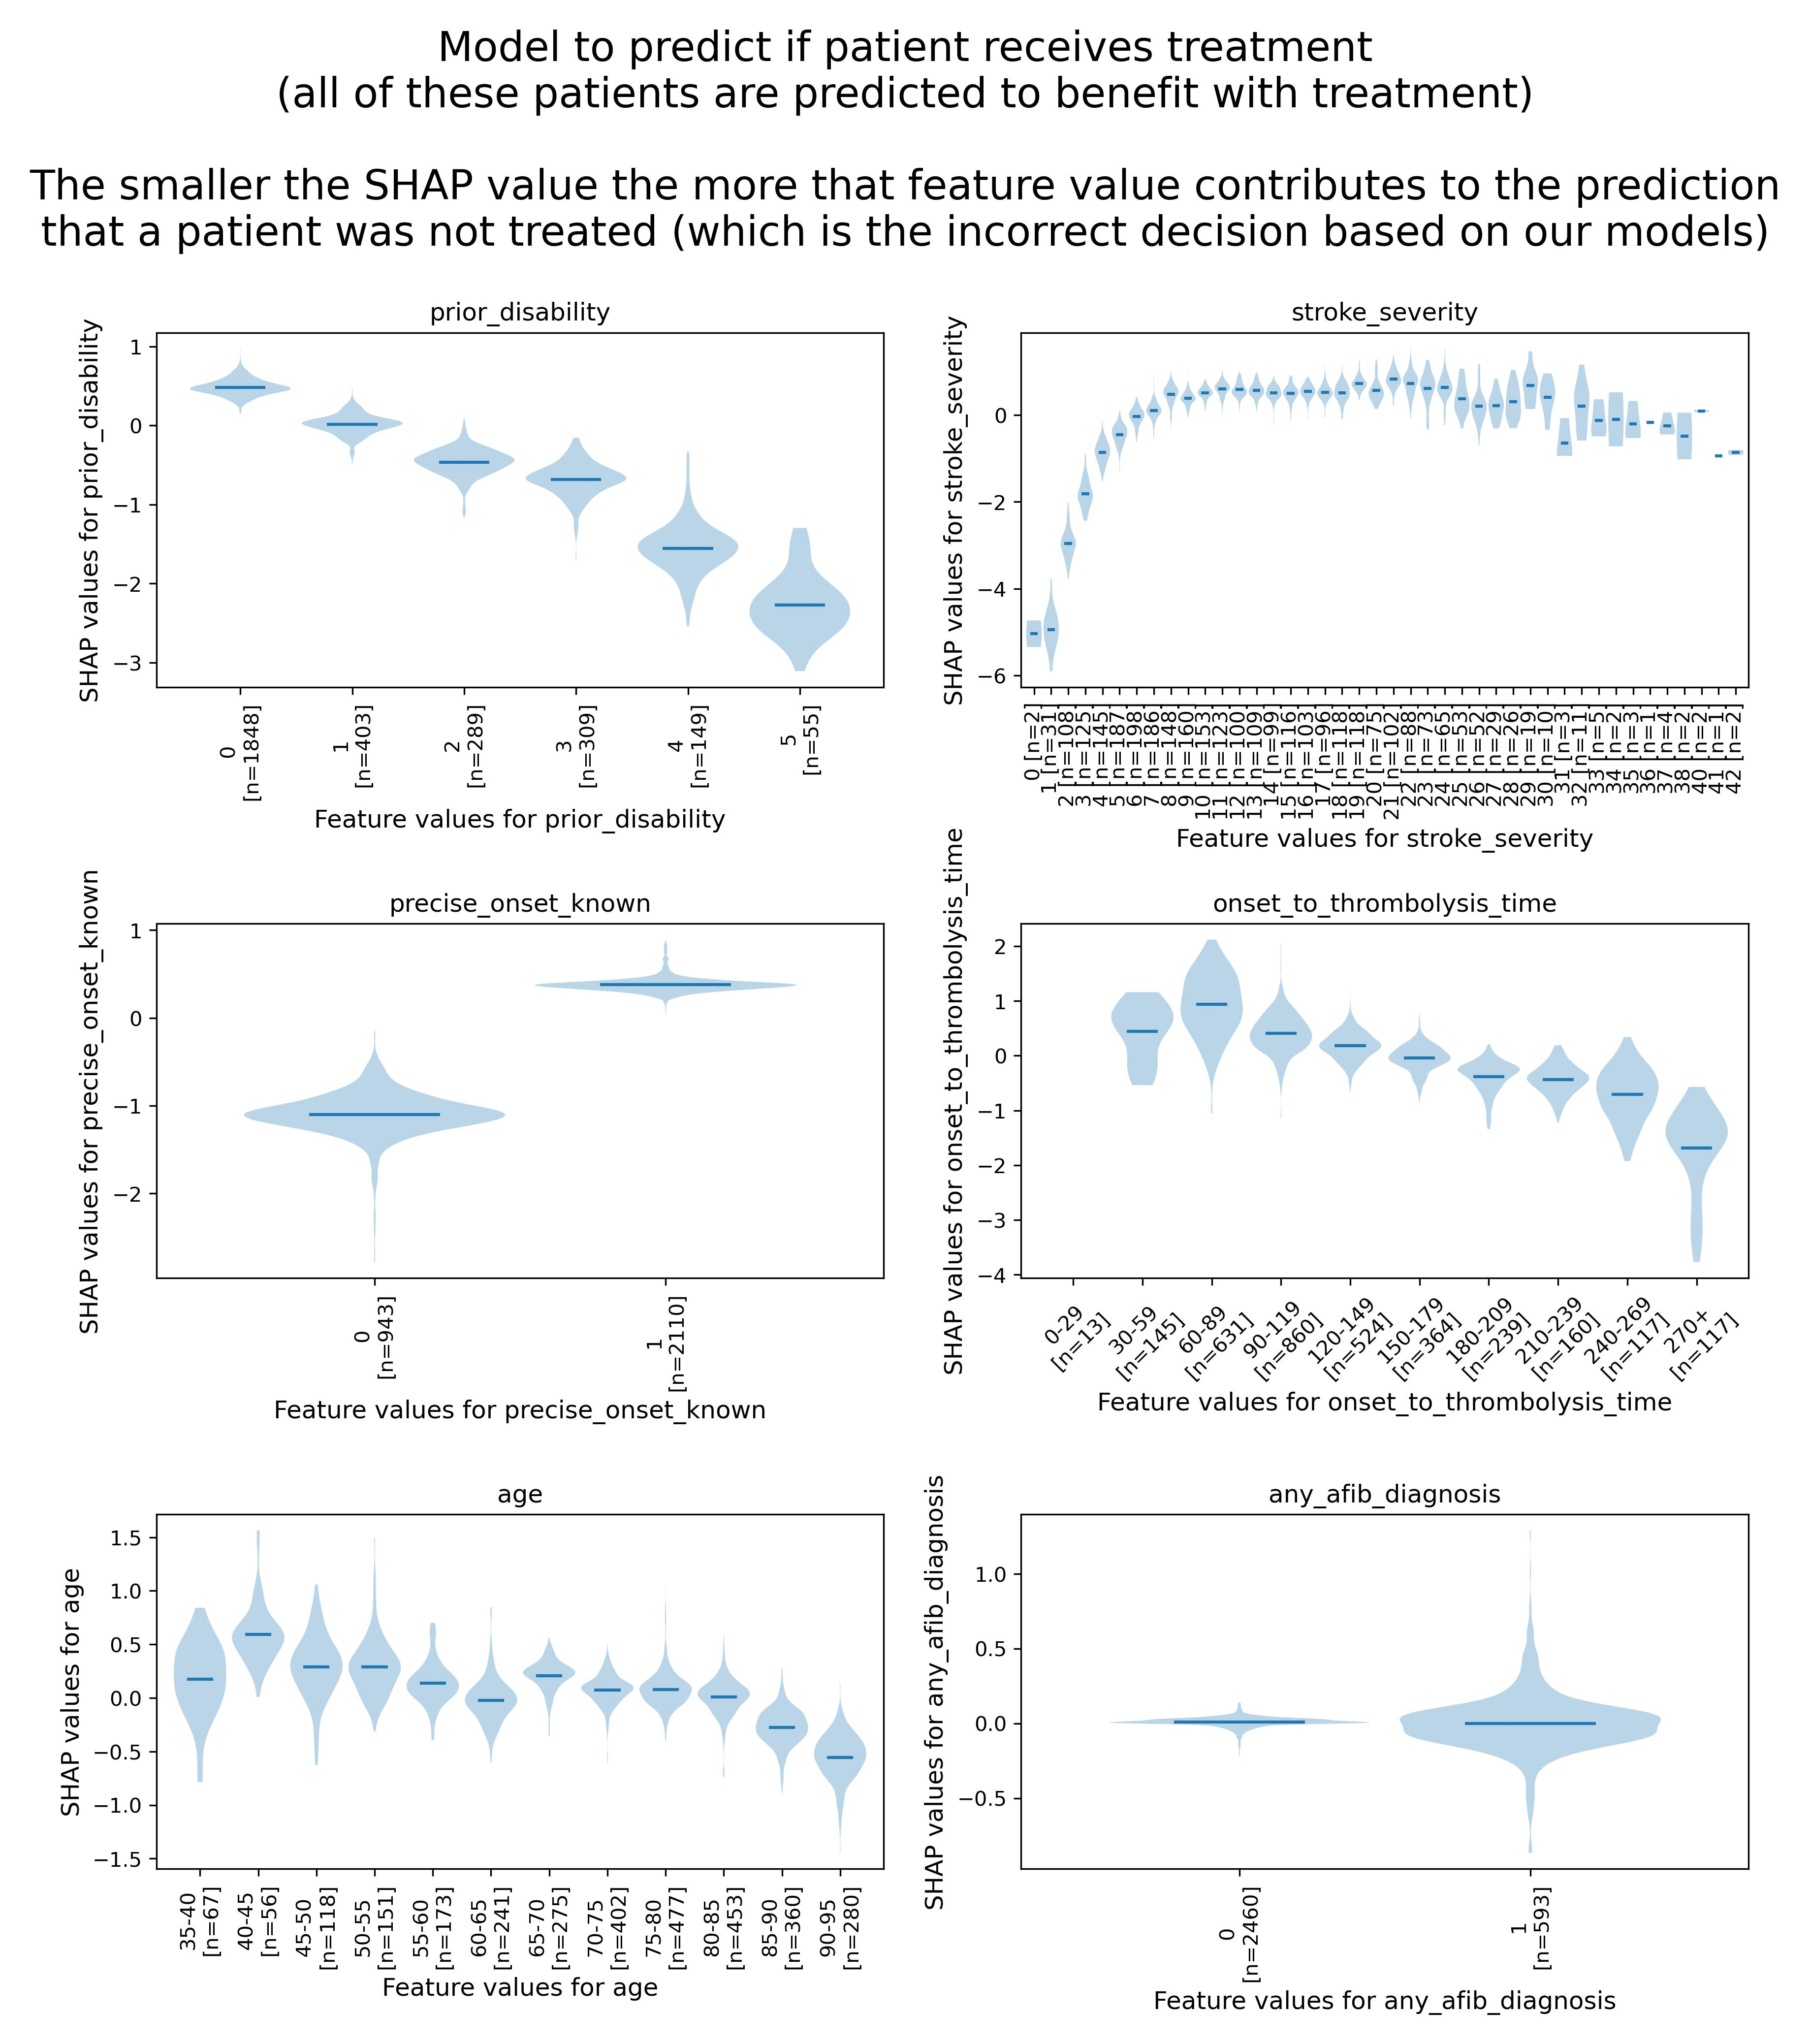
\includegraphics[trim={0 0 0 5cm}, clip, width=0.95\linewidth]    {./images/210_xgb_all_data_multiclass_outcome_999999_shap_violin_all_features_all_benefit_with_ivt}\\
      \label{fig:mrs_violin}
    \end{subfigure}%ults
    \begin{subfigure}{.5\textwidth}
      \centering
      \captionsetup{width=.9\linewidth}
      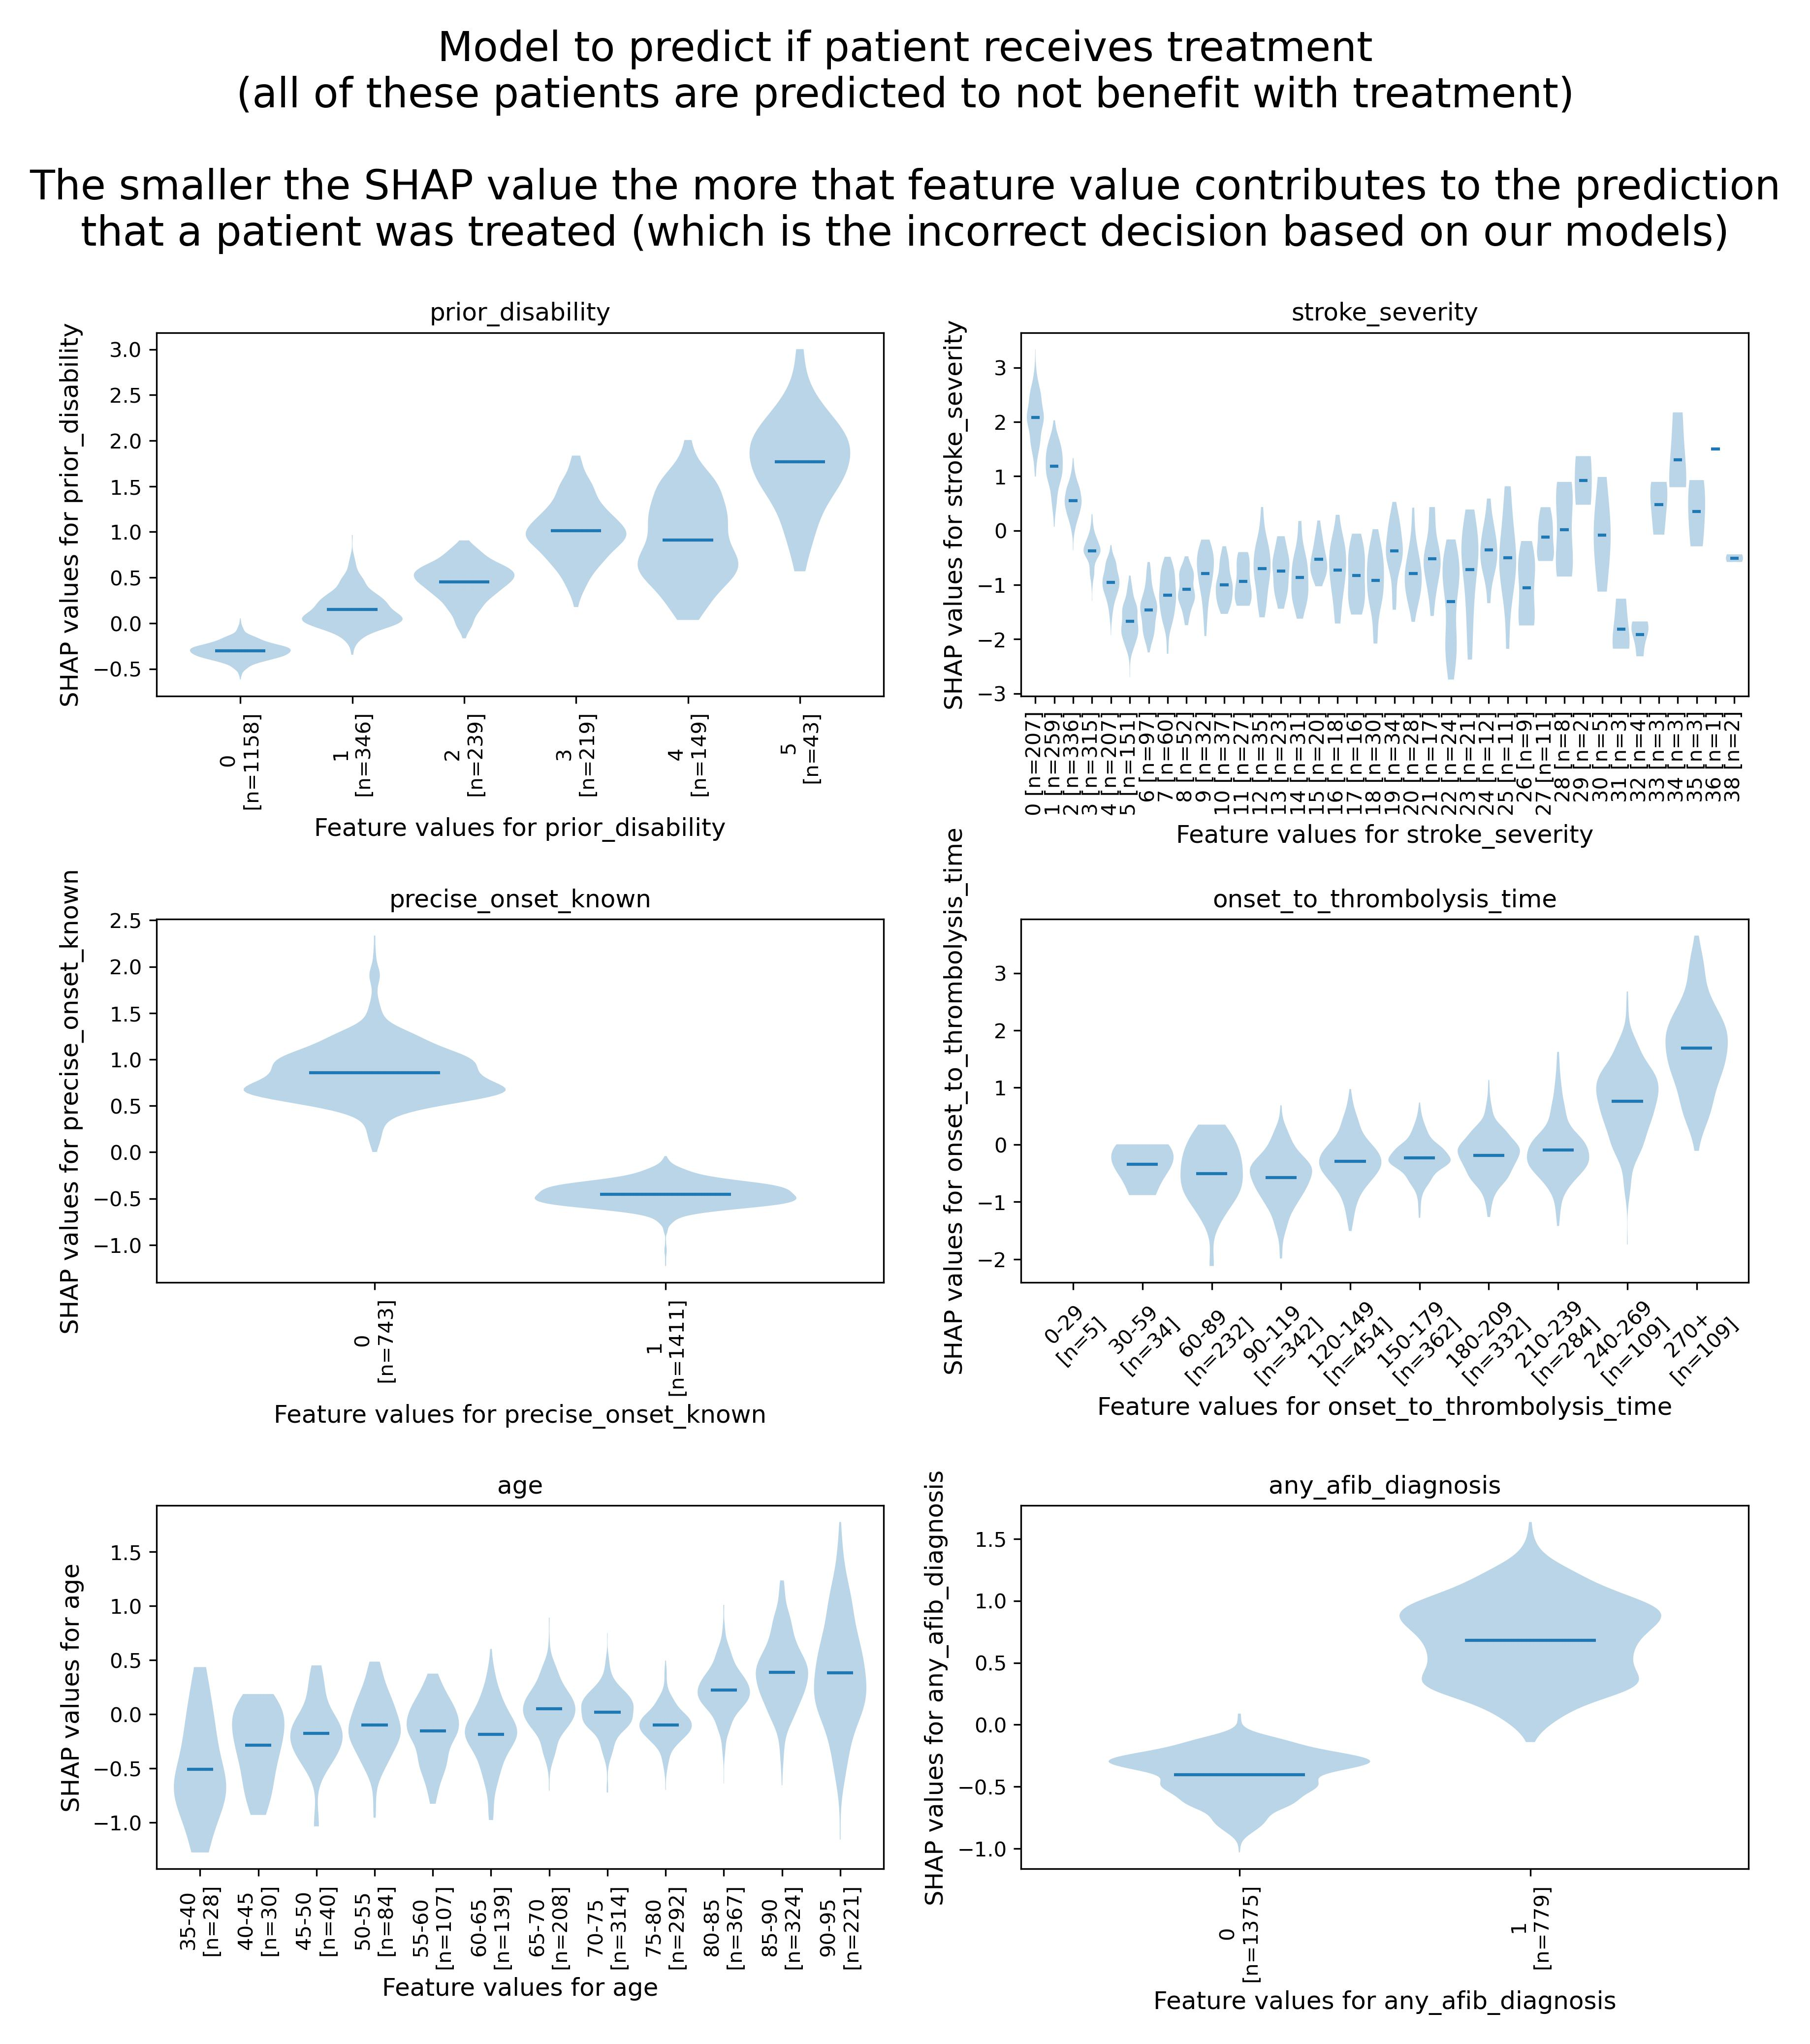
\includegraphics[trim={0 0 0 5cm}, clip, width=0.95\linewidth]{./images/210_xgb_all_data_multiclass_outcome_999999_shap_violin_all_features_none_benefit_with_ivt}\\%{./images/053_predict_mrs6_split_by_ss.png}\\
%        \caption{Predict the likelihood of death on discharge (mRS 6)}
        \label{fig:mrs6_violin_split}
    \end{subfigure}
    \hfill
    \begin{subfigure}{.5\textwidth}
      \centering
      \captionsetup{width=.9\linewidth}
      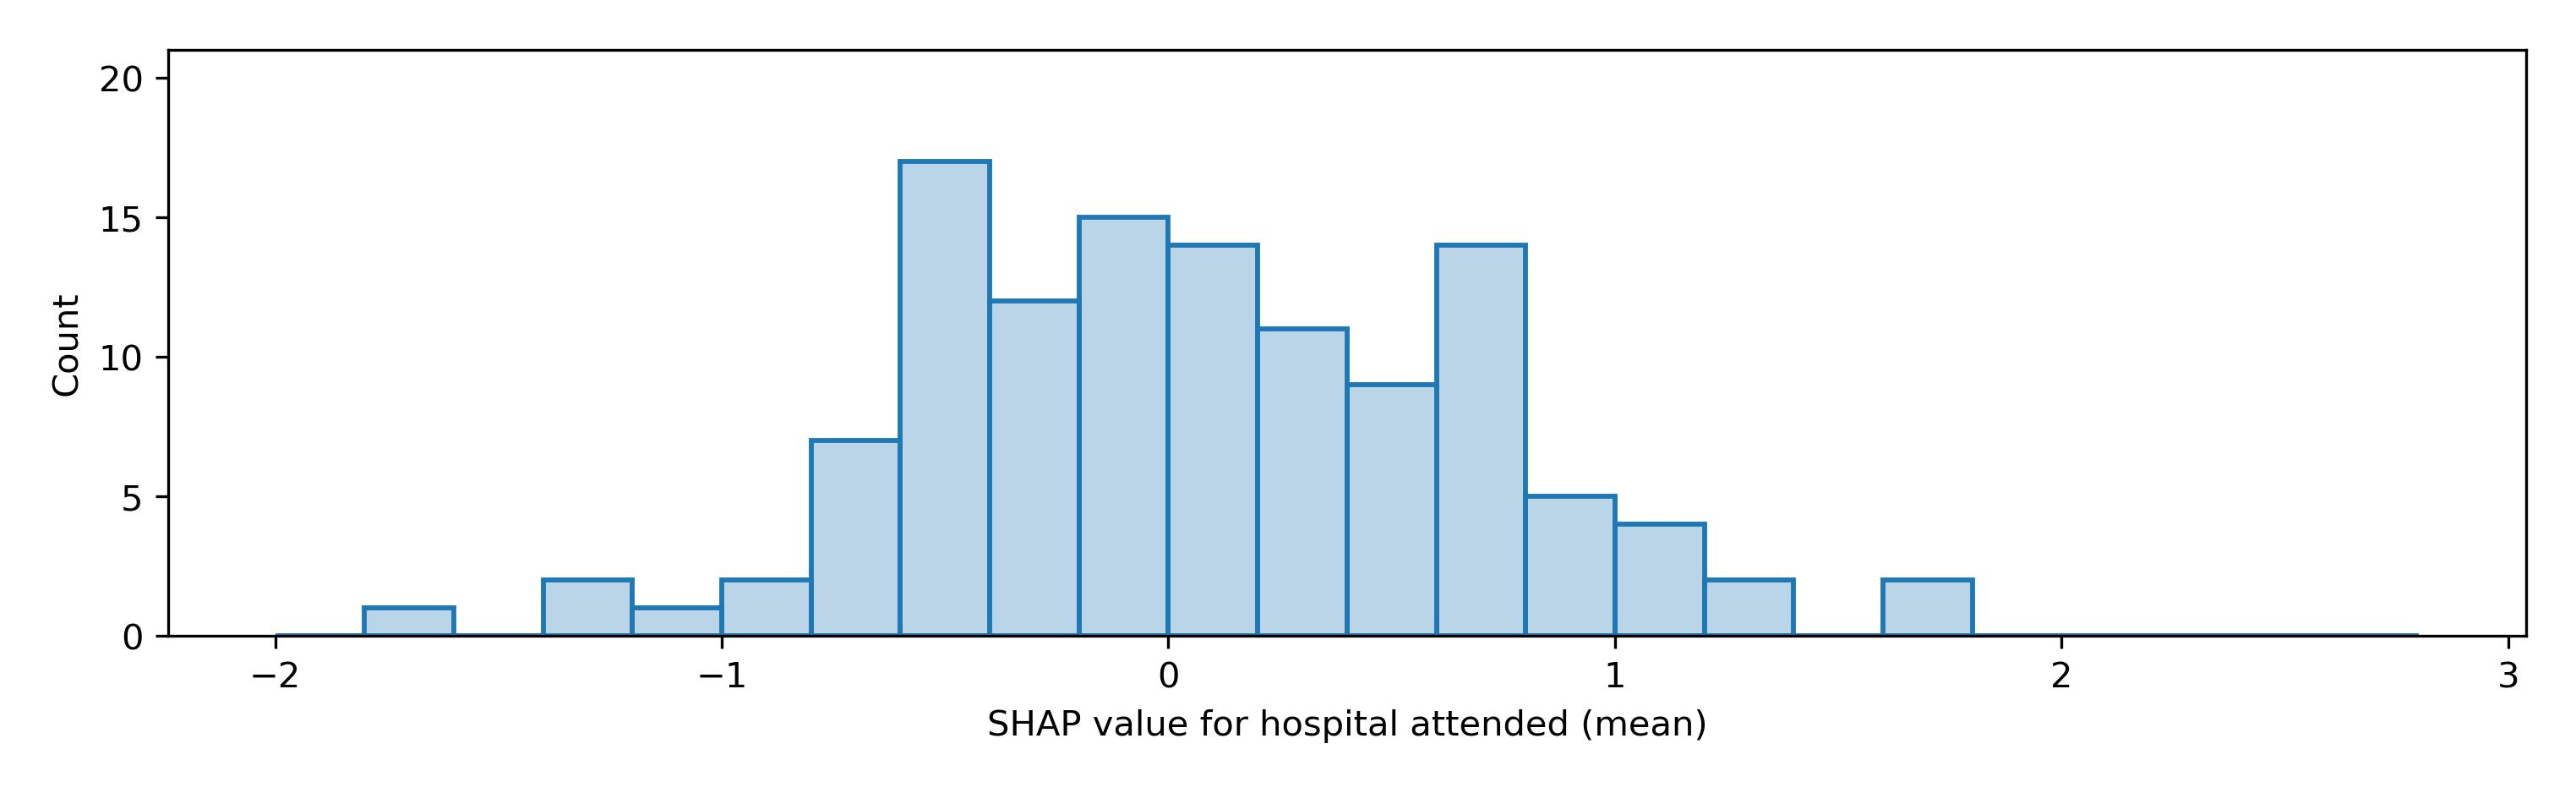
\includegraphics[trim={0 0 0 0.1cm}, clip, width=1\linewidth]    {./images/210_xgb_all_data_multiclass_outcome_999999_hosp_shap_hist_should}\\
      \caption{Predicting correct treatment option for patients that are predicted to benefit with thrombolysis.}
      \label{fig:shap_matching_treatment_should}
    \end{subfigure}%ults
    \begin{subfigure}{.5\textwidth}
      \centering
      \captionsetup{width=.9\linewidth}
      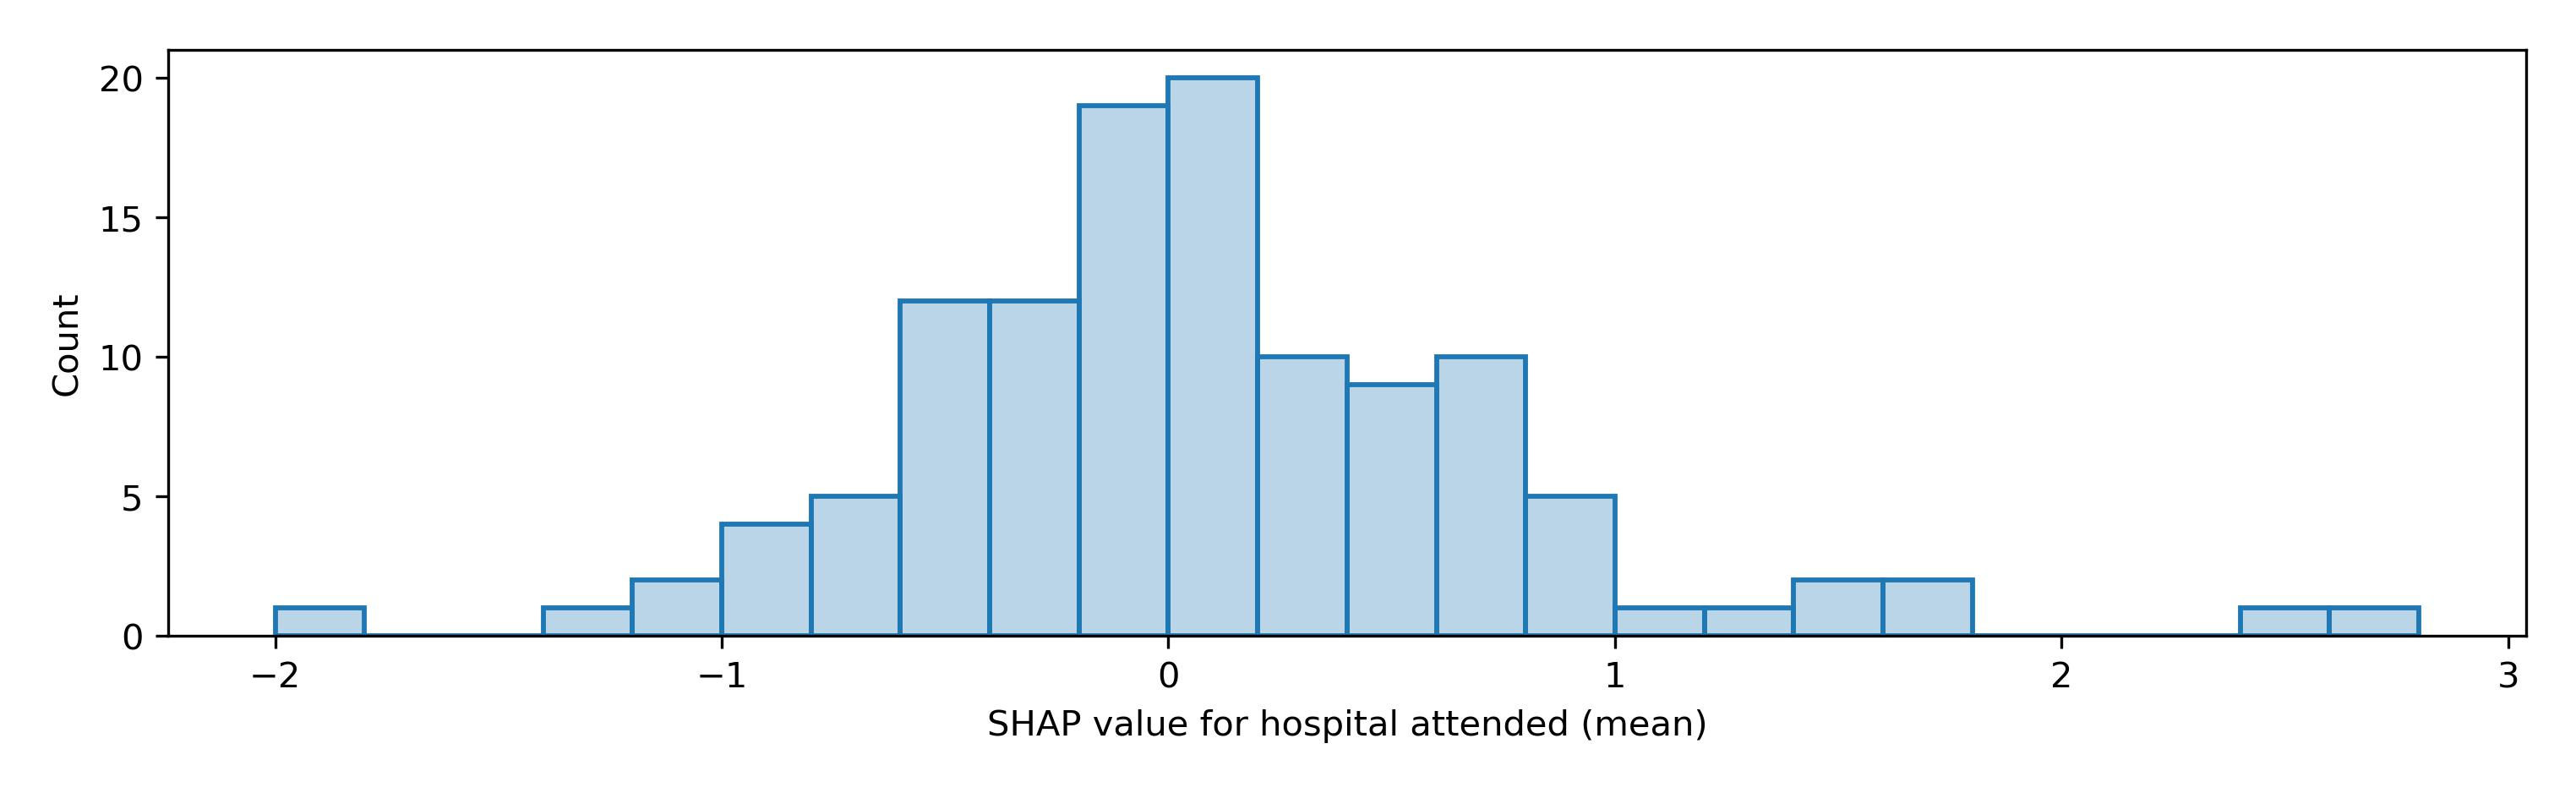
\includegraphics[trim={0 0 0 0.1cm}, clip, width=1\linewidth]
{./images/210_xgb_all_data_multiclass_outcome_999999_hosp_shap_hist_should not}\\
      \caption{Predicting correct treatment option for patients that are predicted to not benefit with thrombolysis}
      \label{fig:shap_matching_treatment_should_not}
    \end{subfigure}
  \caption{Plots showing the relationship between SHAP values and feature values. The smaller the SHAP value more that feature values contributes to the incorrect treatment decision (based on our \textit{multiclass outcome} model. Left: Predicting correct treatment option for patients that are predicted to benefit with thrombolysis. Right: Predicting correct treatment option for patients that are predicted to not benefit with thrombolysis. Top: Violin plots showing the relationship between SHAP values and feature values. The horizontal line shows the median SHAP value. Bottom: Histogram showing the frequency of the mean SHAP value for the hospital attended.}
  \label{fig:shap_matching_treatment}
\end{figure}
\fi

From results section for the sens spec:

In order to compare decisions between hospitals we predicted use of thrombolysis, and outcome with and without thrombolysis, for all of our cohort of 15,680 patients at all hospitals. In order to perform this analysis we built a model to predict whether thrombolysis would be used for each patient at each hospital using XGBoost as previously described \cite{pearn_what_2023}. The XGBoost \textit{thrombolysis decision} model had an accuracy of 78.7\% and ROC-AUC of 0.86 (see supplementary material for more details). For each stroke team we calculated the \textit{Sensitivity} (proportion of patients who were predicted to benefit from thrombolysis who were predicted to receive thrombolysis) and \textit{specificity} (proportion of patients who were predicted not to benefit from thrombolysis who were predicted not to receive thrombolysis) of treatment. 
